\documentclass[twoside]{book}

% Packages required by doxygen
\usepackage{fixltx2e}
\usepackage{calc}
\usepackage{doxygen}
\usepackage{graphicx}
\usepackage[utf8]{inputenc}
\usepackage{makeidx}
\usepackage{multicol}
\usepackage{multirow}
\PassOptionsToPackage{warn}{textcomp}
\usepackage{textcomp}
\usepackage[nointegrals]{wasysym}
\usepackage[table]{xcolor}

% Font selection
\usepackage[T1]{fontenc}
\usepackage{mathptmx}
\usepackage[scaled=.90]{helvet}
\usepackage{courier}
\usepackage{amssymb}
\usepackage{sectsty}
\renewcommand{\familydefault}{\sfdefault}
\allsectionsfont{%
  \fontseries{bc}\selectfont%
  \color{darkgray}%
}
\renewcommand{\DoxyLabelFont}{%
  \fontseries{bc}\selectfont%
  \color{darkgray}%
}
\newcommand{\+}{\discretionary{\mbox{\scriptsize$\hookleftarrow$}}{}{}}

% Page & text layout
\usepackage{geometry}
\geometry{%
  a4paper,%
  top=2.5cm,%
  bottom=2.5cm,%
  left=2.5cm,%
  right=2.5cm%
}
\tolerance=750
\hfuzz=15pt
\hbadness=750
\setlength{\emergencystretch}{15pt}
\setlength{\parindent}{0cm}
\setlength{\parskip}{0.2cm}
\makeatletter
\renewcommand{\paragraph}{%
  \@startsection{paragraph}{4}{0ex}{-1.0ex}{1.0ex}{%
    \normalfont\normalsize\bfseries\SS@parafont%
  }%
}
\renewcommand{\subparagraph}{%
  \@startsection{subparagraph}{5}{0ex}{-1.0ex}{1.0ex}{%
    \normalfont\normalsize\bfseries\SS@subparafont%
  }%
}
\makeatother

% Headers & footers
\usepackage{fancyhdr}
\pagestyle{fancyplain}
\fancyhead[LE]{\fancyplain{}{\bfseries\thepage}}
\fancyhead[CE]{\fancyplain{}{}}
\fancyhead[RE]{\fancyplain{}{\bfseries\leftmark}}
\fancyhead[LO]{\fancyplain{}{\bfseries\rightmark}}
\fancyhead[CO]{\fancyplain{}{}}
\fancyhead[RO]{\fancyplain{}{\bfseries\thepage}}
\fancyfoot[LE]{\fancyplain{}{}}
\fancyfoot[CE]{\fancyplain{}{}}
\fancyfoot[RE]{\fancyplain{}{\bfseries\scriptsize Generated on Mon Oct 20 2014 02\+:48\+:04 for Critter\+Group\+Generator by Doxygen }}
\fancyfoot[LO]{\fancyplain{}{\bfseries\scriptsize Generated on Mon Oct 20 2014 02\+:48\+:04 for Critter\+Group\+Generator by Doxygen }}
\fancyfoot[CO]{\fancyplain{}{}}
\fancyfoot[RO]{\fancyplain{}{}}
\renewcommand{\footrulewidth}{0.4pt}
\renewcommand{\chaptermark}[1]{%
  \markboth{#1}{}%
}
\renewcommand{\sectionmark}[1]{%
  \markright{\thesection\ #1}%
}

% Indices & bibliography
\usepackage{natbib}
\usepackage[titles]{tocloft}
\setcounter{tocdepth}{3}
\setcounter{secnumdepth}{5}
\makeindex

% Hyperlinks (required, but should be loaded last)
\usepackage{ifpdf}
\ifpdf
  \usepackage[pdftex,pagebackref=true]{hyperref}
\else
  \usepackage[ps2pdf,pagebackref=true]{hyperref}
\fi
\hypersetup{%
  colorlinks=true,%
  linkcolor=blue,%
  citecolor=blue,%
  unicode%
}

% Custom commands
\newcommand{\clearemptydoublepage}{%
  \newpage{\pagestyle{empty}\cleardoublepage}%
}


%===== C O N T E N T S =====

\begin{document}

% Titlepage & ToC
\hypersetup{pageanchor=false,
             bookmarks=true,
             bookmarksnumbered=true,
             pdfencoding=unicode
            }
\pagenumbering{roman}
\begin{titlepage}
\vspace*{7cm}
\begin{center}%
{\Large Critter\+Group\+Generator }\\
\vspace*{1cm}
{\large Generated by Doxygen 1.8.8}\\
\vspace*{0.5cm}
{\small Mon Oct 20 2014 02:48:04}\\
\end{center}
\end{titlepage}
\clearemptydoublepage
\tableofcontents
\clearemptydoublepage
\pagenumbering{arabic}
\hypersetup{pageanchor=true}

%--- Begin generated contents ---
\chapter{Hierarchical Index}
\section{Class Hierarchy}
This inheritance list is sorted roughly, but not completely, alphabetically\+:\begin{DoxyCompactList}
\item \contentsline{section}{Map\+:\+:Cell}{\pageref{struct_map_1_1_cell}}{}
\begin{DoxyCompactList}
\item \contentsline{section}{Map\+:\+:Exit\+Cell}{\pageref{struct_map_1_1_exit_cell}}{}
\item \contentsline{section}{Map\+:\+:Path\+Cell}{\pageref{struct_map_1_1_path_cell}}{}
\item \contentsline{section}{Map\+:\+:Scenery\+Cell}{\pageref{struct_map_1_1_scenery_cell}}{}
\item \contentsline{section}{Map\+:\+:Start\+Cell}{\pageref{struct_map_1_1_start_cell}}{}
\item \contentsline{section}{Map\+:\+:Tower\+Cell}{\pageref{struct_map_1_1_tower_cell}}{}
\end{DoxyCompactList}
\item \contentsline{section}{Critter}{\pageref{class_critter}}{}
\begin{DoxyCompactList}
\item \contentsline{section}{Cat}{\pageref{class_cat}}{}
\item \contentsline{section}{Dog}{\pageref{class_dog}}{}
\item \contentsline{section}{Werecat}{\pageref{class_werecat}}{}
\item \contentsline{section}{Werewolf}{\pageref{class_werewolf}}{}
\end{DoxyCompactList}
\item \contentsline{section}{Critter\+Factory}{\pageref{class_critter_factory}}{}
\item \contentsline{section}{Critter\+Wave}{\pageref{class_critter_wave}}{}
\item \contentsline{section}{Critter\+Wave\+:\+:Critter\+Wave\+Deallocator}{\pageref{struct_critter_wave_1_1_critter_wave_deallocator}}{}
\item \contentsline{section}{Map}{\pageref{class_map}}{}
\item \contentsline{section}{Player}{\pageref{class_player}}{}
\end{DoxyCompactList}

\chapter{Class Index}
\section{Class List}
Here are the classes, structs, unions and interfaces with brief descriptions\+:\begin{DoxyCompactList}
\item\contentsline{section}{\hyperlink{class_cat}{Cat} \\*Class for \hyperlink{class_cat}{Cat}. Subclass of \hyperlink{class_critter}{Critter} }{\pageref{class_cat}}{}
\item\contentsline{section}{\hyperlink{struct_map_1_1_cell}{Map\+::\+Cell} \\*Base struct for \hyperlink{struct_map_1_1_cell}{Cell} objects in a \hyperlink{class_map}{Map} }{\pageref{struct_map_1_1_cell}}{}
\item\contentsline{section}{\hyperlink{class_critter}{Critter} \\*Abstract base class of all Critters \hyperlink{class_critter}{Critter} defines the attributes, accessors, and update function for its subclass instances }{\pageref{class_critter}}{}
\item\contentsline{section}{\hyperlink{class_critter_factory}{Critter\+Factory} \\*Creates objects derived from \hyperlink{class_critter}{Critter}. Utility class that creates instance of a \hyperlink{class_critter}{Critter} subclass from a family of derived \hyperlink{class_critter}{Critter} classes }{\pageref{class_critter_factory}}{}
\item\contentsline{section}{\hyperlink{class_critter_wave}{Critter\+Wave} \\*Represents a wave of Critters. Class that has holds Critters in a map data structure, which represents a wave of Critters }{\pageref{class_critter_wave}}{}
\item\contentsline{section}{\hyperlink{struct_critter_wave_1_1_critter_wave_deallocator}{Critter\+Wave\+::\+Critter\+Wave\+Deallocator} \\*Struct deallocating resources used in a \hyperlink{class_critter_wave}{Critter\+Wave} map }{\pageref{struct_critter_wave_1_1_critter_wave_deallocator}}{}
\item\contentsline{section}{\hyperlink{class_dog}{Dog} \\*Class for \hyperlink{class_dog}{Dog}. Subclass of \hyperlink{class_critter}{Critter} }{\pageref{class_dog}}{}
\item\contentsline{section}{\hyperlink{struct_map_1_1_exit_cell}{Map\+::\+Exit\+Cell} \\*Derived from base struct \hyperlink{struct_map_1_1_cell}{Cell} }{\pageref{struct_map_1_1_exit_cell}}{}
\item\contentsline{section}{\hyperlink{class_map}{Map} \\*Class for \hyperlink{class_map}{Map}. Stub class of map for Critters }{\pageref{class_map}}{}
\item\contentsline{section}{\hyperlink{struct_map_1_1_path_cell}{Map\+::\+Path\+Cell} \\*Derived from base struct \hyperlink{struct_map_1_1_cell}{Cell} }{\pageref{struct_map_1_1_path_cell}}{}
\item\contentsline{section}{\hyperlink{class_player}{Player} \\*Class for \hyperlink{class_player}{Player}. Stub class of \hyperlink{class_player}{Player} for Critters }{\pageref{class_player}}{}
\item\contentsline{section}{\hyperlink{struct_map_1_1_scenery_cell}{Map\+::\+Scenery\+Cell} \\*Derived from base struct \hyperlink{struct_map_1_1_cell}{Cell} }{\pageref{struct_map_1_1_scenery_cell}}{}
\item\contentsline{section}{\hyperlink{struct_map_1_1_start_cell}{Map\+::\+Start\+Cell} \\*Derived from base struct \hyperlink{struct_map_1_1_cell}{Cell} }{\pageref{struct_map_1_1_start_cell}}{}
\item\contentsline{section}{\hyperlink{struct_map_1_1_tower_cell}{Map\+::\+Tower\+Cell} \\*Derived from base struct \hyperlink{struct_map_1_1_cell}{Cell} }{\pageref{struct_map_1_1_tower_cell}}{}
\item\contentsline{section}{\hyperlink{class_werecat}{Werecat} \\*Class for \hyperlink{class_werecat}{Werecat}. Subclass of \hyperlink{class_critter}{Critter} }{\pageref{class_werecat}}{}
\item\contentsline{section}{\hyperlink{class_werewolf}{Werewolf} \\*Class for \hyperlink{class_werewolf}{Werewolf}. Subclass of \hyperlink{class_critter}{Critter} }{\pageref{class_werewolf}}{}
\end{DoxyCompactList}

\chapter{File Index}
\section{File List}
Here is a list of all files with brief descriptions\+:\begin{DoxyCompactList}
\item\contentsline{section}{C\+O\+M\+P345/\+Assignment1\+\_\+no\+G\+U\+I/\+Critter\+Group\+Generator/\+Critter\+Group\+Generator/include/\hyperlink{_cat_8h}{Cat.\+h} \\*Representation of \hyperlink{class_cat}{Cat} object }{\pageref{_cat_8h}}{}
\item\contentsline{section}{C\+O\+M\+P345/\+Assignment1\+\_\+no\+G\+U\+I/\+Critter\+Group\+Generator/\+Critter\+Group\+Generator/include/\hyperlink{_critter_8h}{Critter.\+h} \\*Representation of critter object }{\pageref{_critter_8h}}{}
\item\contentsline{section}{C\+O\+M\+P345/\+Assignment1\+\_\+no\+G\+U\+I/\+Critter\+Group\+Generator/\+Critter\+Group\+Generator/include/\hyperlink{_critter_factory_8h}{Critter\+Factory.\+h} \\*File for \hyperlink{class_critter_factory}{Critter\+Factory} class }{\pageref{_critter_factory_8h}}{}
\item\contentsline{section}{C\+O\+M\+P345/\+Assignment1\+\_\+no\+G\+U\+I/\+Critter\+Group\+Generator/\+Critter\+Group\+Generator/include/\hyperlink{_critter_wave_8h}{Critter\+Wave.\+h} \\*File for \hyperlink{class_critter_wave}{Critter\+Wave} class }{\pageref{_critter_wave_8h}}{}
\item\contentsline{section}{C\+O\+M\+P345/\+Assignment1\+\_\+no\+G\+U\+I/\+Critter\+Group\+Generator/\+Critter\+Group\+Generator/include/\hyperlink{_dog_8h}{Dog.\+h} \\*Representation of \hyperlink{class_dog}{Dog} object }{\pageref{_dog_8h}}{}
\item\contentsline{section}{C\+O\+M\+P345/\+Assignment1\+\_\+no\+G\+U\+I/\+Critter\+Group\+Generator/\+Critter\+Group\+Generator/include/\hyperlink{_map_8h}{Map.\+h} \\*Representation of \hyperlink{class_map}{Map} object }{\pageref{_map_8h}}{}
\item\contentsline{section}{C\+O\+M\+P345/\+Assignment1\+\_\+no\+G\+U\+I/\+Critter\+Group\+Generator/\+Critter\+Group\+Generator/include/\hyperlink{_player_8h}{Player.\+h} \\*Representation of \hyperlink{class_player}{Player} object }{\pageref{_player_8h}}{}
\item\contentsline{section}{C\+O\+M\+P345/\+Assignment1\+\_\+no\+G\+U\+I/\+Critter\+Group\+Generator/\+Critter\+Group\+Generator/include/\hyperlink{_werecat_8h}{Werecat.\+h} \\*Representation of \hyperlink{class_werecat}{Werecat} object }{\pageref{_werecat_8h}}{}
\item\contentsline{section}{C\+O\+M\+P345/\+Assignment1\+\_\+no\+G\+U\+I/\+Critter\+Group\+Generator/\+Critter\+Group\+Generator/include/\hyperlink{_werewolf_8h}{Werewolf.\+h} \\*Representation of \hyperlink{class_werewolf}{Werewolf} object }{\pageref{_werewolf_8h}}{}
\item\contentsline{section}{C\+O\+M\+P345/\+Assignment1\+\_\+no\+G\+U\+I/\+Critter\+Group\+Generator/\+Critter\+Group\+Generator/src/\hyperlink{_driver_8cpp}{Driver.\+cpp} }{\pageref{_driver_8cpp}}{}
\item\contentsline{section}{C\+O\+M\+P345/\+Assignment1\+\_\+no\+G\+U\+I/\+Critter\+Group\+Generator/\+Critter\+Group\+Generator/src/game\+Objects/\hyperlink{_cat_8cpp}{Cat.\+cpp} }{\pageref{_cat_8cpp}}{}
\item\contentsline{section}{C\+O\+M\+P345/\+Assignment1\+\_\+no\+G\+U\+I/\+Critter\+Group\+Generator/\+Critter\+Group\+Generator/src/game\+Objects/\hyperlink{_critter_8cpp}{Critter.\+cpp} }{\pageref{_critter_8cpp}}{}
\item\contentsline{section}{C\+O\+M\+P345/\+Assignment1\+\_\+no\+G\+U\+I/\+Critter\+Group\+Generator/\+Critter\+Group\+Generator/src/game\+Objects/\hyperlink{_critter_factory_8cpp}{Critter\+Factory.\+cpp} }{\pageref{_critter_factory_8cpp}}{}
\item\contentsline{section}{C\+O\+M\+P345/\+Assignment1\+\_\+no\+G\+U\+I/\+Critter\+Group\+Generator/\+Critter\+Group\+Generator/src/game\+Objects/\hyperlink{_critter_wave_8cpp}{Critter\+Wave.\+cpp} }{\pageref{_critter_wave_8cpp}}{}
\item\contentsline{section}{C\+O\+M\+P345/\+Assignment1\+\_\+no\+G\+U\+I/\+Critter\+Group\+Generator/\+Critter\+Group\+Generator/src/game\+Objects/\hyperlink{_dog_8cpp}{Dog.\+cpp} }{\pageref{_dog_8cpp}}{}
\item\contentsline{section}{C\+O\+M\+P345/\+Assignment1\+\_\+no\+G\+U\+I/\+Critter\+Group\+Generator/\+Critter\+Group\+Generator/src/game\+Objects/\hyperlink{_werecat_8cpp}{Werecat.\+cpp} }{\pageref{_werecat_8cpp}}{}
\item\contentsline{section}{C\+O\+M\+P345/\+Assignment1\+\_\+no\+G\+U\+I/\+Critter\+Group\+Generator/\+Critter\+Group\+Generator/src/game\+Objects/\hyperlink{_werewolf_8cpp}{Werewolf.\+cpp} }{\pageref{_werewolf_8cpp}}{}
\end{DoxyCompactList}

\chapter{Class Documentation}
\hypertarget{class_cat}{\section{Cat Class Reference}
\label{class_cat}\index{Cat@{Cat}}
}


Class for \hyperlink{class_cat}{Cat}. Subclass of \hyperlink{class_critter}{Critter}.  




{\ttfamily \#include $<$Cat.\+h$>$}



Inheritance diagram for Cat\+:
\nopagebreak
\begin{figure}[H]
\begin{center}
\leavevmode
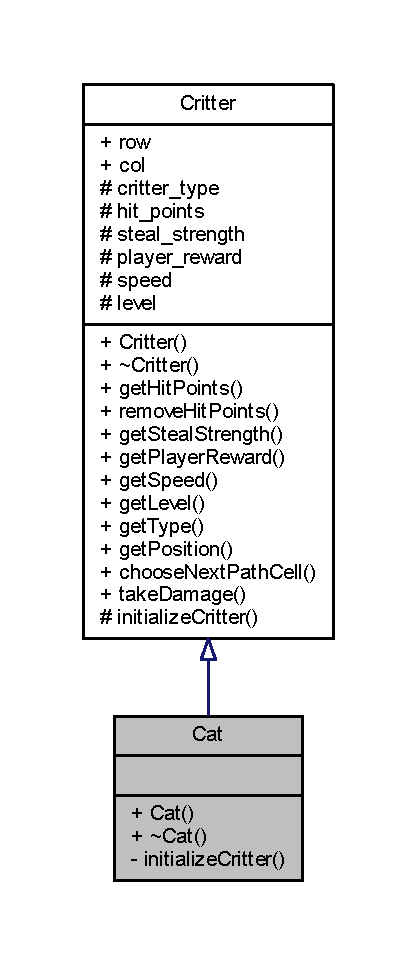
\includegraphics[width=200pt]{class_cat__inherit__graph}
\end{center}
\end{figure}


Collaboration diagram for Cat\+:
\nopagebreak
\begin{figure}[H]
\begin{center}
\leavevmode
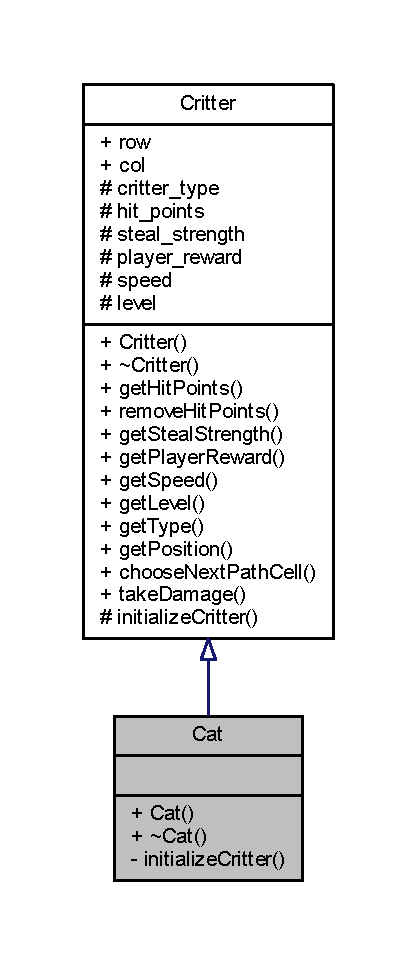
\includegraphics[width=200pt]{class_cat__coll__graph}
\end{center}
\end{figure}
\subsection*{Public Member Functions}
\begin{DoxyCompactItemize}
\item 
\hyperlink{class_cat_adff0d67c4d14c4eeeb35b8daa33ee442}{Cat} ()
\begin{DoxyCompactList}\small\item\em The \hyperlink{class_cat}{Cat} constructor. Calls \hyperlink{class_cat_a2bf5faec9a7399c19e6dceb9402a34d7}{initialize\+Critter()} to set attributes of the \hyperlink{class_cat}{Cat} object. \end{DoxyCompactList}\item 
\hyperlink{class_cat_accae87693b84127a716243cbf5e6ddee}{$\sim$\+Cat} ()
\end{DoxyCompactItemize}
\subsection*{Private Member Functions}
\begin{DoxyCompactItemize}
\item 
virtual void \hyperlink{class_cat_a2bf5faec9a7399c19e6dceb9402a34d7}{initialize\+Critter} ()
\begin{DoxyCompactList}\small\item\em Initialization function for a \hyperlink{class_cat}{Cat}. \end{DoxyCompactList}\end{DoxyCompactItemize}
\subsection*{Additional Inherited Members}


\subsection{Detailed Description}
Class for \hyperlink{class_cat}{Cat}. Subclass of \hyperlink{class_critter}{Critter}. 

\subsection{Constructor \& Destructor Documentation}
\hypertarget{class_cat_adff0d67c4d14c4eeeb35b8daa33ee442}{\index{Cat@{Cat}!Cat@{Cat}}
\index{Cat@{Cat}!Cat@{Cat}}
\subsubsection[{Cat}]{\setlength{\rightskip}{0pt plus 5cm}Cat\+::\+Cat (
\begin{DoxyParamCaption}
{}
\end{DoxyParamCaption}
)}}\label{class_cat_adff0d67c4d14c4eeeb35b8daa33ee442}


The \hyperlink{class_cat}{Cat} constructor. Calls \hyperlink{class_cat_a2bf5faec9a7399c19e6dceb9402a34d7}{initialize\+Critter()} to set attributes of the \hyperlink{class_cat}{Cat} object. 



Here is the call graph for this function\+:
\nopagebreak
\begin{figure}[H]
\begin{center}
\leavevmode
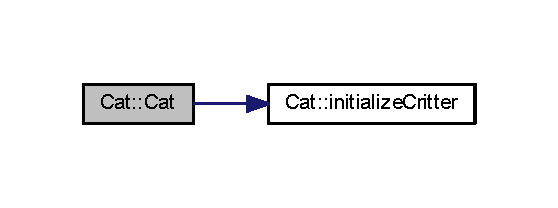
\includegraphics[width=268pt]{class_cat_adff0d67c4d14c4eeeb35b8daa33ee442_cgraph}
\end{center}
\end{figure}


\hypertarget{class_cat_accae87693b84127a716243cbf5e6ddee}{\index{Cat@{Cat}!````~Cat@{$\sim$\+Cat}}
\index{````~Cat@{$\sim$\+Cat}!Cat@{Cat}}
\subsubsection[{$\sim$\+Cat}]{\setlength{\rightskip}{0pt plus 5cm}Cat\+::$\sim$\+Cat (
\begin{DoxyParamCaption}
{}
\end{DoxyParamCaption}
)\hspace{0.3cm}{\ttfamily [inline]}}}\label{class_cat_accae87693b84127a716243cbf5e6ddee}


\subsection{Member Function Documentation}
\hypertarget{class_cat_a2bf5faec9a7399c19e6dceb9402a34d7}{\index{Cat@{Cat}!initialize\+Critter@{initialize\+Critter}}
\index{initialize\+Critter@{initialize\+Critter}!Cat@{Cat}}
\subsubsection[{initialize\+Critter}]{\setlength{\rightskip}{0pt plus 5cm}void Cat\+::initialize\+Critter (
\begin{DoxyParamCaption}
{}
\end{DoxyParamCaption}
)\hspace{0.3cm}{\ttfamily [private]}, {\ttfamily [virtual]}}}\label{class_cat_a2bf5faec9a7399c19e6dceb9402a34d7}


Initialization function for a \hyperlink{class_cat}{Cat}. 

\begin{DoxyReturn}{Returns}
Void.
\end{DoxyReturn}
Initialization specific to a \hyperlink{class_cat}{Cat} object 

Implements \hyperlink{class_critter_ab903f6d28ef3fc70808390fef8816b79}{Critter}.



Here is the caller graph for this function\+:
\nopagebreak
\begin{figure}[H]
\begin{center}
\leavevmode
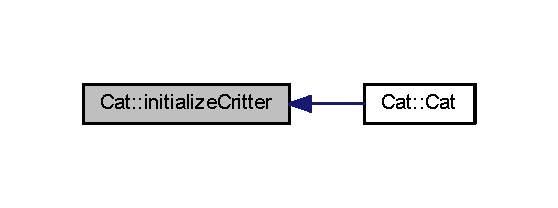
\includegraphics[width=268pt]{class_cat_a2bf5faec9a7399c19e6dceb9402a34d7_icgraph}
\end{center}
\end{figure}




The documentation for this class was generated from the following files\+:\begin{DoxyCompactItemize}
\item 
C\+O\+M\+P345/\+Assignment1\+\_\+no\+G\+U\+I/\+Critter\+Group\+Generator/\+Critter\+Group\+Generator/include/\hyperlink{_cat_8h}{Cat.\+h}\item 
C\+O\+M\+P345/\+Assignment1\+\_\+no\+G\+U\+I/\+Critter\+Group\+Generator/\+Critter\+Group\+Generator/src/game\+Objects/\hyperlink{_cat_8cpp}{Cat.\+cpp}\end{DoxyCompactItemize}

\hypertarget{struct_map_1_1_cell}{\section{Map\+:\+:Cell Struct Reference}
\label{struct_map_1_1_cell}\index{Map\+::\+Cell@{Map\+::\+Cell}}
}


Base struct for \hyperlink{struct_map_1_1_cell}{Cell} objects in a \hyperlink{class_map}{Map}.  




{\ttfamily \#include $<$Map.\+h$>$}



Inheritance diagram for Map\+:\+:Cell\+:
\nopagebreak
\begin{figure}[H]
\begin{center}
\leavevmode
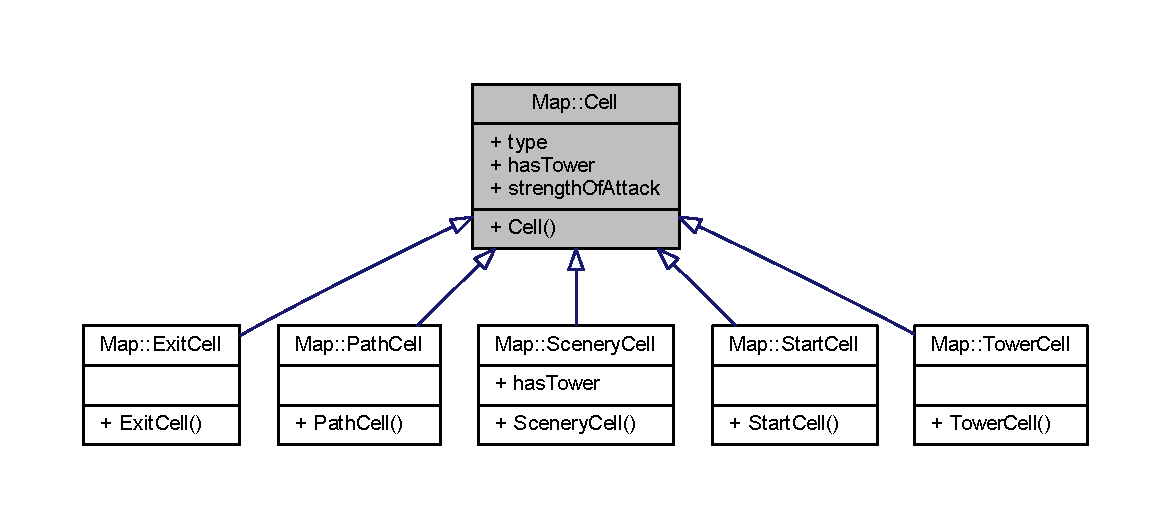
\includegraphics[width=350pt]{struct_map_1_1_cell__inherit__graph}
\end{center}
\end{figure}


Collaboration diagram for Map\+:\+:Cell\+:
\nopagebreak
\begin{figure}[H]
\begin{center}
\leavevmode
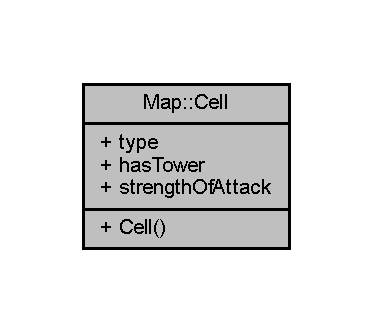
\includegraphics[width=179pt]{struct_map_1_1_cell__coll__graph}
\end{center}
\end{figure}
\subsection*{Public Member Functions}
\begin{DoxyCompactItemize}
\item 
\hyperlink{struct_map_1_1_cell_a1264b2260fee132a303effb0f95aab02}{Cell} ()
\end{DoxyCompactItemize}
\subsection*{Public Attributes}
\begin{DoxyCompactItemize}
\item 
\hyperlink{class_map_a25b1781a19b5a600a92f0487b823b272}{Cell\+Type} \hyperlink{struct_map_1_1_cell_adab6ad663eeda4c1fe349ea2f87598e0}{type}
\item 
bool \hyperlink{struct_map_1_1_cell_a3f2e341ce722e5f95ae4ddb2db1b7164}{has\+Tower}
\item 
int \hyperlink{struct_map_1_1_cell_a46cdedee9b275a54df5fbf6c1e18650b}{strength\+Of\+Attack}
\end{DoxyCompactItemize}


\subsection{Detailed Description}
Base struct for \hyperlink{struct_map_1_1_cell}{Cell} objects in a \hyperlink{class_map}{Map}. 

\subsection{Constructor \& Destructor Documentation}
\hypertarget{struct_map_1_1_cell_a1264b2260fee132a303effb0f95aab02}{\index{Map\+::\+Cell@{Map\+::\+Cell}!Cell@{Cell}}
\index{Cell@{Cell}!Map\+::\+Cell@{Map\+::\+Cell}}
\subsubsection[{Cell}]{\setlength{\rightskip}{0pt plus 5cm}Map\+::\+Cell\+::\+Cell (
\begin{DoxyParamCaption}
{}
\end{DoxyParamCaption}
)\hspace{0.3cm}{\ttfamily [inline]}}}\label{struct_map_1_1_cell_a1264b2260fee132a303effb0f95aab02}


\subsection{Member Data Documentation}
\hypertarget{struct_map_1_1_cell_a3f2e341ce722e5f95ae4ddb2db1b7164}{\index{Map\+::\+Cell@{Map\+::\+Cell}!has\+Tower@{has\+Tower}}
\index{has\+Tower@{has\+Tower}!Map\+::\+Cell@{Map\+::\+Cell}}
\subsubsection[{has\+Tower}]{\setlength{\rightskip}{0pt plus 5cm}bool Map\+::\+Cell\+::has\+Tower}}\label{struct_map_1_1_cell_a3f2e341ce722e5f95ae4ddb2db1b7164}
\hypertarget{struct_map_1_1_cell_a46cdedee9b275a54df5fbf6c1e18650b}{\index{Map\+::\+Cell@{Map\+::\+Cell}!strength\+Of\+Attack@{strength\+Of\+Attack}}
\index{strength\+Of\+Attack@{strength\+Of\+Attack}!Map\+::\+Cell@{Map\+::\+Cell}}
\subsubsection[{strength\+Of\+Attack}]{\setlength{\rightskip}{0pt plus 5cm}int Map\+::\+Cell\+::strength\+Of\+Attack}}\label{struct_map_1_1_cell_a46cdedee9b275a54df5fbf6c1e18650b}
\hypertarget{struct_map_1_1_cell_adab6ad663eeda4c1fe349ea2f87598e0}{\index{Map\+::\+Cell@{Map\+::\+Cell}!type@{type}}
\index{type@{type}!Map\+::\+Cell@{Map\+::\+Cell}}
\subsubsection[{type}]{\setlength{\rightskip}{0pt plus 5cm}{\bf Cell\+Type} Map\+::\+Cell\+::type}}\label{struct_map_1_1_cell_adab6ad663eeda4c1fe349ea2f87598e0}


The documentation for this struct was generated from the following file\+:\begin{DoxyCompactItemize}
\item 
C\+O\+M\+P345/\+Assignment1\+\_\+no\+G\+U\+I/\+Critter\+Group\+Generator/\+Critter\+Group\+Generator/include/\hyperlink{_map_8h}{Map.\+h}\end{DoxyCompactItemize}

\hypertarget{class_critter}{\section{Critter Class Reference}
\label{class_critter}\index{Critter@{Critter}}
}


Abstract base class of all Critters \hyperlink{class_critter}{Critter} defines the attributes, accessors, and update function for its subclass instances.  




{\ttfamily \#include $<$Critter.\+h$>$}



Inheritance diagram for Critter\+:
\nopagebreak
\begin{figure}[H]
\begin{center}
\leavevmode
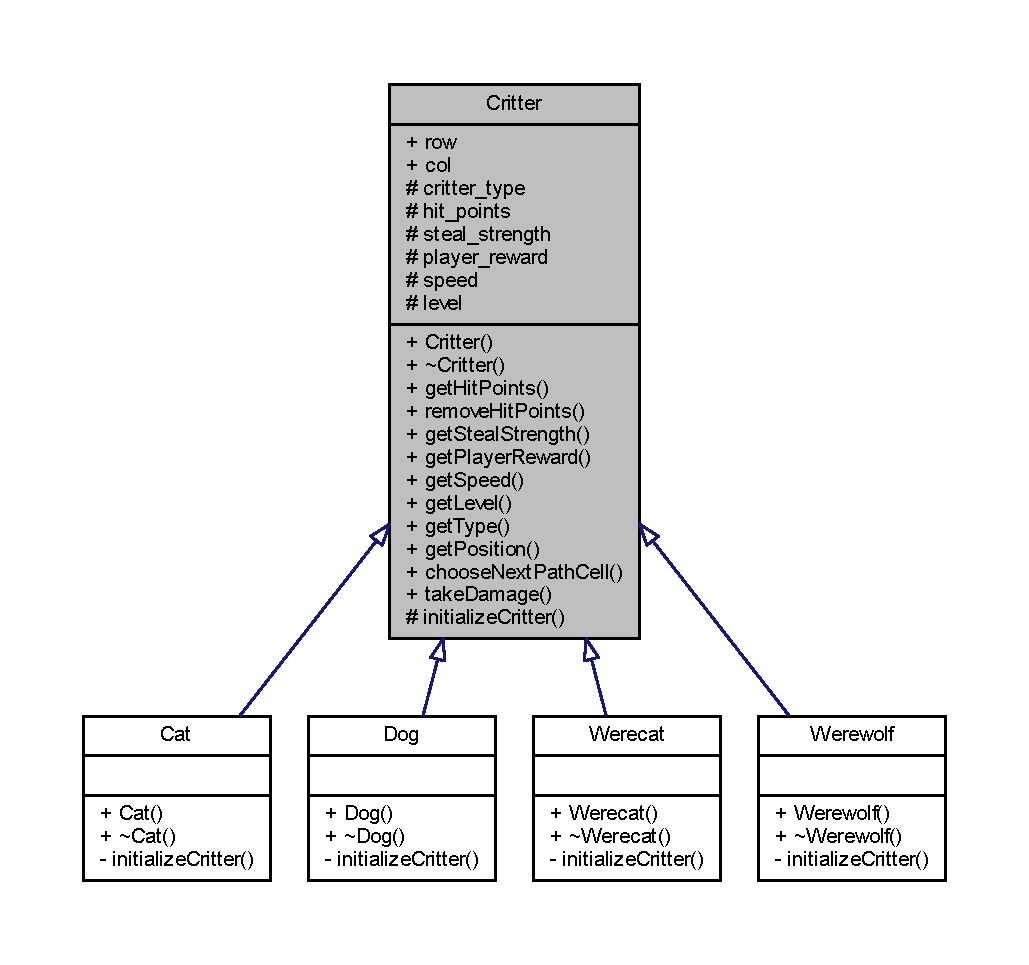
\includegraphics[width=350pt]{class_critter__inherit__graph}
\end{center}
\end{figure}


Collaboration diagram for Critter\+:
\nopagebreak
\begin{figure}[H]
\begin{center}
\leavevmode
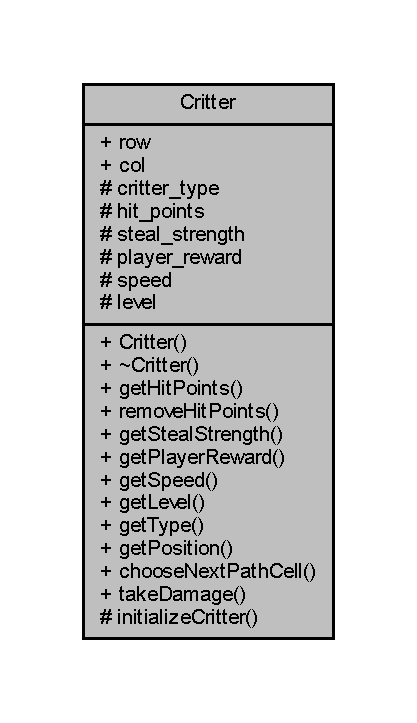
\includegraphics[width=200pt]{class_critter__coll__graph}
\end{center}
\end{figure}
\subsection*{Public Member Functions}
\begin{DoxyCompactItemize}
\item 
\hyperlink{class_critter_a05aa21e3b570d7380f3ead47c99442ef}{Critter} ()
\item 
virtual \hyperlink{class_critter_aa923c19cdc302c7bf10a038983e801c1}{$\sim$\+Critter} ()
\item 
int \hyperlink{class_critter_a1e98c05f5a41102cc37eb7a4396b90cf}{get\+Hit\+Points} () const 
\item 
void \hyperlink{class_critter_a3d18092d84c66b53adfbc480c3ce1b42}{remove\+Hit\+Points} (int points)
\item 
int \hyperlink{class_critter_a18a43eb5bca5c6bd0113eca15723c625}{get\+Steal\+Strength} () const 
\item 
int \hyperlink{class_critter_a7db2281b14479a1c931716c07acbc7da}{get\+Player\+Reward} () const 
\item 
float \hyperlink{class_critter_a3785ffa05cec86b30264fbdbf613e4f8}{get\+Speed} () const 
\item 
int \hyperlink{class_critter_aebbb372bdcd3a709428445554c3d24c9}{get\+Level} () const 
\item 
std\+::string \hyperlink{class_critter_a47b5b7e7544429f5913605bedbfb9a63}{get\+Type} () const 
\item 
std\+::string \hyperlink{class_critter_a51bd0c313d265926c561517783f4b598}{get\+Position} () const 
\item 
void \hyperlink{class_critter_acda941387ac28fc3e7e4ce92a864997e}{choose\+Next\+Path\+Cell} (\hyperlink{class_map}{Map} \&map, int current\+\_\+row, int current\+\_\+col, \hyperlink{class_player}{Player} \&player)
\begin{DoxyCompactList}\small\item\em Picks the next path cell to go to. \end{DoxyCompactList}\item 
void \hyperlink{class_critter_a963ccea758c0b04129a372572704c1fc}{take\+Damage} (int damage)
\begin{DoxyCompactList}\small\item\em Handles the damage taken by a \hyperlink{class_critter}{Critter} in range of a Tower. \end{DoxyCompactList}\end{DoxyCompactItemize}
\subsection*{Public Attributes}
\begin{DoxyCompactItemize}
\item 
int \hyperlink{class_critter_aec02dae27ba8081064ac2b035eaf82cf}{row}
\item 
int \hyperlink{class_critter_a22fc3dd912a58aafc3aa7f118f1f2440}{col}
\end{DoxyCompactItemize}
\subsection*{Protected Member Functions}
\begin{DoxyCompactItemize}
\item 
virtual void \hyperlink{class_critter_ab903f6d28ef3fc70808390fef8816b79}{initialize\+Critter} ()=0
\begin{DoxyCompactList}\small\item\em Pure virtualized initialization function for \hyperlink{class_critter}{Critter}. \end{DoxyCompactList}\end{DoxyCompactItemize}
\subsection*{Protected Attributes}
\begin{DoxyCompactItemize}
\item 
std\+::string \hyperlink{class_critter_a0228568729f86823591b390f53ad5ebc}{critter\+\_\+type}
\begin{DoxyCompactList}\small\item\em Type of the \hyperlink{class_critter}{Critter}. \end{DoxyCompactList}\item 
int \hyperlink{class_critter_a916038a11e8443ea403a644e91fc791e}{hit\+\_\+points}
\begin{DoxyCompactList}\small\item\em Health of the \hyperlink{class_critter}{Critter}. \end{DoxyCompactList}\item 
int \hyperlink{class_critter_a60f7c436aec1f6a63d4fb5af57eb8eef}{steal\+\_\+strength}
\begin{DoxyCompactList}\small\item\em Rate at which the critter can steal coins from the player. \end{DoxyCompactList}\item 
int \hyperlink{class_critter_a2a17f7366fbde83714742e66ba3e63a7}{player\+\_\+reward}
\begin{DoxyCompactList}\small\item\em Coin reward for the player when the \hyperlink{class_critter}{Critter} is killed. \end{DoxyCompactList}\item 
float \hyperlink{class_critter_adde7d84a0dd9ac8f5dc144464928638f}{speed}
\begin{DoxyCompactList}\small\item\em \hyperlink{class_critter}{Critter} movement speed. \end{DoxyCompactList}\item 
int \hyperlink{class_critter_a9f9a6408a55212036f317710dc3da410}{level}
\begin{DoxyCompactList}\small\item\em Difficulty level as part of a wave. \end{DoxyCompactList}\end{DoxyCompactItemize}
\subsection*{Friends}
\begin{DoxyCompactItemize}
\item 
std\+::ostream \& \hyperlink{class_critter_aeed4299a358eceabb3abc2ba9ec83ef2}{operator$<$$<$} (std\+::ostream \&output, const \hyperlink{class_critter}{Critter} \&critter)
\begin{DoxyCompactList}\small\item\em Overloaded cout operator to print out Critters. \end{DoxyCompactList}\end{DoxyCompactItemize}


\subsection{Detailed Description}
Abstract base class of all Critters \hyperlink{class_critter}{Critter} defines the attributes, accessors, and update function for its subclass instances. 

\subsection{Constructor \& Destructor Documentation}
\hypertarget{class_critter_a05aa21e3b570d7380f3ead47c99442ef}{\index{Critter@{Critter}!Critter@{Critter}}
\index{Critter@{Critter}!Critter@{Critter}}
\subsubsection[{Critter}]{\setlength{\rightskip}{0pt plus 5cm}Critter\+::\+Critter (
\begin{DoxyParamCaption}
{}
\end{DoxyParamCaption}
)\hspace{0.3cm}{\ttfamily [inline]}}}\label{class_critter_a05aa21e3b570d7380f3ead47c99442ef}
\hypertarget{class_critter_aa923c19cdc302c7bf10a038983e801c1}{\index{Critter@{Critter}!````~Critter@{$\sim$\+Critter}}
\index{````~Critter@{$\sim$\+Critter}!Critter@{Critter}}
\subsubsection[{$\sim$\+Critter}]{\setlength{\rightskip}{0pt plus 5cm}virtual Critter\+::$\sim$\+Critter (
\begin{DoxyParamCaption}
{}
\end{DoxyParamCaption}
)\hspace{0.3cm}{\ttfamily [inline]}, {\ttfamily [virtual]}}}\label{class_critter_aa923c19cdc302c7bf10a038983e801c1}


\subsection{Member Function Documentation}
\hypertarget{class_critter_acda941387ac28fc3e7e4ce92a864997e}{\index{Critter@{Critter}!choose\+Next\+Path\+Cell@{choose\+Next\+Path\+Cell}}
\index{choose\+Next\+Path\+Cell@{choose\+Next\+Path\+Cell}!Critter@{Critter}}
\subsubsection[{choose\+Next\+Path\+Cell}]{\setlength{\rightskip}{0pt plus 5cm}void Critter\+::choose\+Next\+Path\+Cell (
\begin{DoxyParamCaption}
\item[{{\bf Map} \&}]{map, }
\item[{int}]{current\+\_\+row, }
\item[{int}]{current\+\_\+col, }
\item[{{\bf Player} \&}]{player}
\end{DoxyParamCaption}
)}}\label{class_critter_acda941387ac28fc3e7e4ce92a864997e}


Picks the next path cell to go to. 


\begin{DoxyParams}{Parameters}
{\em map} & \hyperlink{class_map}{Map} reference. \\
\hline
{\em current\+\_\+row} & Current row of \hyperlink{class_critter}{Critter} position. \\
\hline
{\em current\+\_\+col} & Current column of \hyperlink{class_critter}{Critter} position. \\
\hline
\end{DoxyParams}
\begin{DoxyReturn}{Returns}
Void.
\end{DoxyReturn}
This function goes through every cell in the map, looking for the next path or exit cell. The search begins at the critter's current position, which is passed in. If the next path cell is found, the \hyperlink{class_critter}{Critter}'s position (row and column) is updated to that cell. If the the exit is reached, the critter steals coins from the player. 

Here is the call graph for this function\+:
\nopagebreak
\begin{figure}[H]
\begin{center}
\leavevmode
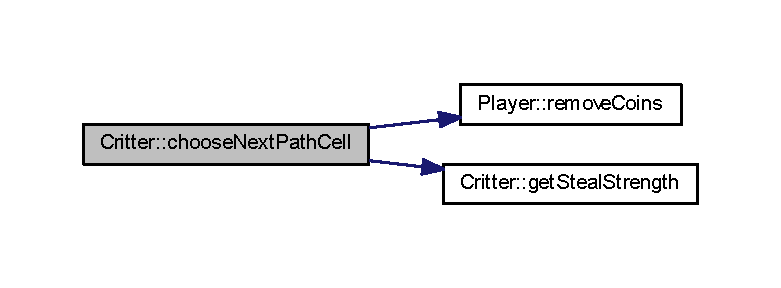
\includegraphics[width=350pt]{class_critter_acda941387ac28fc3e7e4ce92a864997e_cgraph}
\end{center}
\end{figure}




Here is the caller graph for this function\+:
\nopagebreak
\begin{figure}[H]
\begin{center}
\leavevmode
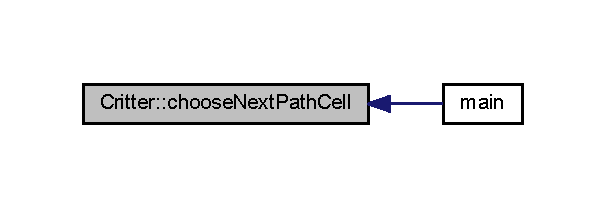
\includegraphics[width=291pt]{class_critter_acda941387ac28fc3e7e4ce92a864997e_icgraph}
\end{center}
\end{figure}


\hypertarget{class_critter_a1e98c05f5a41102cc37eb7a4396b90cf}{\index{Critter@{Critter}!get\+Hit\+Points@{get\+Hit\+Points}}
\index{get\+Hit\+Points@{get\+Hit\+Points}!Critter@{Critter}}
\subsubsection[{get\+Hit\+Points}]{\setlength{\rightskip}{0pt plus 5cm}int Critter\+::get\+Hit\+Points (
\begin{DoxyParamCaption}
{}
\end{DoxyParamCaption}
) const}}\label{class_critter_a1e98c05f5a41102cc37eb7a4396b90cf}


Here is the caller graph for this function\+:
\nopagebreak
\begin{figure}[H]
\begin{center}
\leavevmode
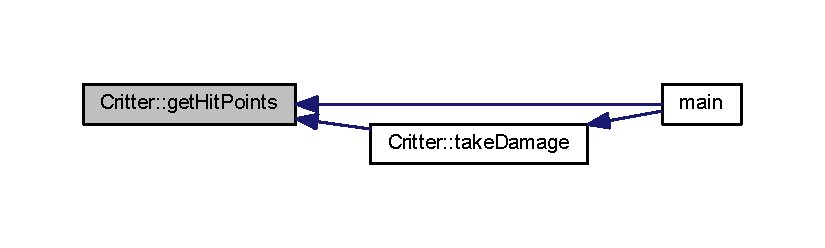
\includegraphics[width=350pt]{class_critter_a1e98c05f5a41102cc37eb7a4396b90cf_icgraph}
\end{center}
\end{figure}


\hypertarget{class_critter_aebbb372bdcd3a709428445554c3d24c9}{\index{Critter@{Critter}!get\+Level@{get\+Level}}
\index{get\+Level@{get\+Level}!Critter@{Critter}}
\subsubsection[{get\+Level}]{\setlength{\rightskip}{0pt plus 5cm}int Critter\+::get\+Level (
\begin{DoxyParamCaption}
{}
\end{DoxyParamCaption}
) const}}\label{class_critter_aebbb372bdcd3a709428445554c3d24c9}
\hypertarget{class_critter_a7db2281b14479a1c931716c07acbc7da}{\index{Critter@{Critter}!get\+Player\+Reward@{get\+Player\+Reward}}
\index{get\+Player\+Reward@{get\+Player\+Reward}!Critter@{Critter}}
\subsubsection[{get\+Player\+Reward}]{\setlength{\rightskip}{0pt plus 5cm}int Critter\+::get\+Player\+Reward (
\begin{DoxyParamCaption}
{}
\end{DoxyParamCaption}
) const}}\label{class_critter_a7db2281b14479a1c931716c07acbc7da}
\hypertarget{class_critter_a51bd0c313d265926c561517783f4b598}{\index{Critter@{Critter}!get\+Position@{get\+Position}}
\index{get\+Position@{get\+Position}!Critter@{Critter}}
\subsubsection[{get\+Position}]{\setlength{\rightskip}{0pt plus 5cm}std\+::string Critter\+::get\+Position (
\begin{DoxyParamCaption}
{}
\end{DoxyParamCaption}
) const}}\label{class_critter_a51bd0c313d265926c561517783f4b598}


Here is the caller graph for this function\+:
\nopagebreak
\begin{figure}[H]
\begin{center}
\leavevmode
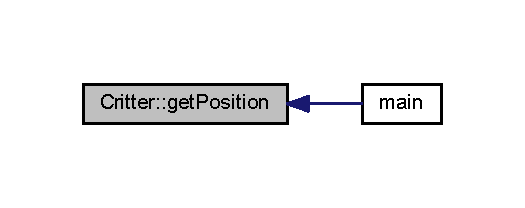
\includegraphics[width=252pt]{class_critter_a51bd0c313d265926c561517783f4b598_icgraph}
\end{center}
\end{figure}


\hypertarget{class_critter_a3785ffa05cec86b30264fbdbf613e4f8}{\index{Critter@{Critter}!get\+Speed@{get\+Speed}}
\index{get\+Speed@{get\+Speed}!Critter@{Critter}}
\subsubsection[{get\+Speed}]{\setlength{\rightskip}{0pt plus 5cm}float Critter\+::get\+Speed (
\begin{DoxyParamCaption}
{}
\end{DoxyParamCaption}
) const}}\label{class_critter_a3785ffa05cec86b30264fbdbf613e4f8}
\hypertarget{class_critter_a18a43eb5bca5c6bd0113eca15723c625}{\index{Critter@{Critter}!get\+Steal\+Strength@{get\+Steal\+Strength}}
\index{get\+Steal\+Strength@{get\+Steal\+Strength}!Critter@{Critter}}
\subsubsection[{get\+Steal\+Strength}]{\setlength{\rightskip}{0pt plus 5cm}int Critter\+::get\+Steal\+Strength (
\begin{DoxyParamCaption}
{}
\end{DoxyParamCaption}
) const}}\label{class_critter_a18a43eb5bca5c6bd0113eca15723c625}


Here is the caller graph for this function\+:
\nopagebreak
\begin{figure}[H]
\begin{center}
\leavevmode
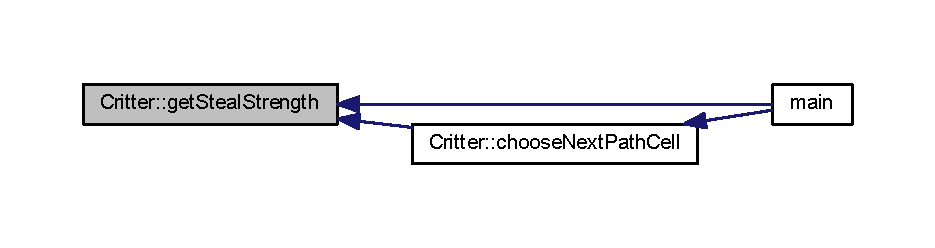
\includegraphics[width=350pt]{class_critter_a18a43eb5bca5c6bd0113eca15723c625_icgraph}
\end{center}
\end{figure}


\hypertarget{class_critter_a47b5b7e7544429f5913605bedbfb9a63}{\index{Critter@{Critter}!get\+Type@{get\+Type}}
\index{get\+Type@{get\+Type}!Critter@{Critter}}
\subsubsection[{get\+Type}]{\setlength{\rightskip}{0pt plus 5cm}std\+::string Critter\+::get\+Type (
\begin{DoxyParamCaption}
{}
\end{DoxyParamCaption}
) const}}\label{class_critter_a47b5b7e7544429f5913605bedbfb9a63}
\hypertarget{class_critter_ab903f6d28ef3fc70808390fef8816b79}{\index{Critter@{Critter}!initialize\+Critter@{initialize\+Critter}}
\index{initialize\+Critter@{initialize\+Critter}!Critter@{Critter}}
\subsubsection[{initialize\+Critter}]{\setlength{\rightskip}{0pt plus 5cm}virtual void Critter\+::initialize\+Critter (
\begin{DoxyParamCaption}
{}
\end{DoxyParamCaption}
)\hspace{0.3cm}{\ttfamily [protected]}, {\ttfamily [pure virtual]}}}\label{class_critter_ab903f6d28ef3fc70808390fef8816b79}


Pure virtualized initialization function for \hyperlink{class_critter}{Critter}. 

\begin{DoxyReturn}{Returns}
Void. 
\end{DoxyReturn}


Implemented in \hyperlink{class_cat_a2bf5faec9a7399c19e6dceb9402a34d7}{Cat}, \hyperlink{class_dog_ab512ed7b74de6ab907e4199f98d82566}{Dog}, \hyperlink{class_werecat_ae3c16d3ee0d96cb7ad7126cc3ae088a0}{Werecat}, and \hyperlink{class_werewolf_afc8553cf4e3e33a609ca08c084d66ce0}{Werewolf}.

\hypertarget{class_critter_a3d18092d84c66b53adfbc480c3ce1b42}{\index{Critter@{Critter}!remove\+Hit\+Points@{remove\+Hit\+Points}}
\index{remove\+Hit\+Points@{remove\+Hit\+Points}!Critter@{Critter}}
\subsubsection[{remove\+Hit\+Points}]{\setlength{\rightskip}{0pt plus 5cm}void Critter\+::remove\+Hit\+Points (
\begin{DoxyParamCaption}
\item[{int}]{points}
\end{DoxyParamCaption}
)}}\label{class_critter_a3d18092d84c66b53adfbc480c3ce1b42}


Here is the caller graph for this function\+:
\nopagebreak
\begin{figure}[H]
\begin{center}
\leavevmode
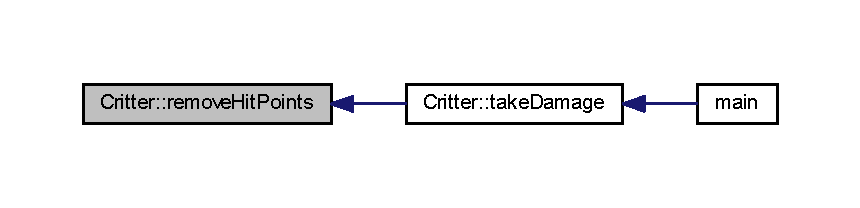
\includegraphics[width=350pt]{class_critter_a3d18092d84c66b53adfbc480c3ce1b42_icgraph}
\end{center}
\end{figure}


\hypertarget{class_critter_a963ccea758c0b04129a372572704c1fc}{\index{Critter@{Critter}!take\+Damage@{take\+Damage}}
\index{take\+Damage@{take\+Damage}!Critter@{Critter}}
\subsubsection[{take\+Damage}]{\setlength{\rightskip}{0pt plus 5cm}void Critter\+::take\+Damage (
\begin{DoxyParamCaption}
\item[{int}]{damage}
\end{DoxyParamCaption}
)}}\label{class_critter_a963ccea758c0b04129a372572704c1fc}


Handles the damage taken by a \hyperlink{class_critter}{Critter} in range of a Tower. 


\begin{DoxyParams}{Parameters}
{\em damage} & Int representing the amount of health lost per hit. \\
\hline
\end{DoxyParams}
\begin{DoxyReturn}{Returns}
Void. 
\end{DoxyReturn}


Here is the call graph for this function\+:
\nopagebreak
\begin{figure}[H]
\begin{center}
\leavevmode
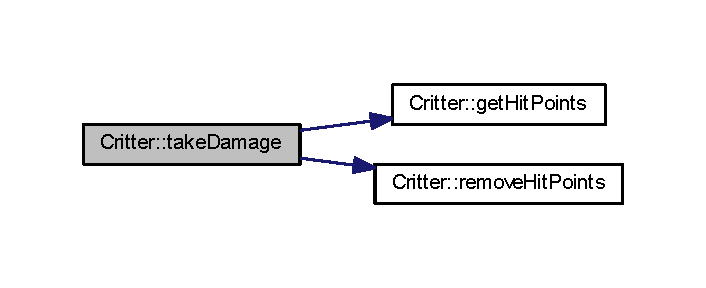
\includegraphics[width=339pt]{class_critter_a963ccea758c0b04129a372572704c1fc_cgraph}
\end{center}
\end{figure}




Here is the caller graph for this function\+:
\nopagebreak
\begin{figure}[H]
\begin{center}
\leavevmode
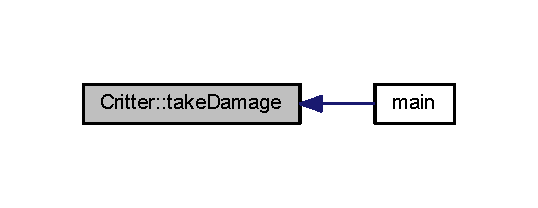
\includegraphics[width=258pt]{class_critter_a963ccea758c0b04129a372572704c1fc_icgraph}
\end{center}
\end{figure}




\subsection{Friends And Related Function Documentation}
\hypertarget{class_critter_aeed4299a358eceabb3abc2ba9ec83ef2}{\index{Critter@{Critter}!operator$<$$<$@{operator$<$$<$}}
\index{operator$<$$<$@{operator$<$$<$}!Critter@{Critter}}
\subsubsection[{operator$<$$<$}]{\setlength{\rightskip}{0pt plus 5cm}std\+::ostream\& operator$<$$<$ (
\begin{DoxyParamCaption}
\item[{std\+::ostream \&}]{output, }
\item[{const {\bf Critter} \&}]{critter}
\end{DoxyParamCaption}
)\hspace{0.3cm}{\ttfamily [friend]}}}\label{class_critter_aeed4299a358eceabb3abc2ba9ec83ef2}


Overloaded cout operator to print out Critters. 


\begin{DoxyParams}{Parameters}
{\em output} & Output stream address \\
\hline
{\em critter} & Const address to \hyperlink{class_critter}{Critter} \\
\hline
\end{DoxyParams}
\begin{DoxyReturn}{Returns}
Address to output stream 
\end{DoxyReturn}


\subsection{Member Data Documentation}
\hypertarget{class_critter_a22fc3dd912a58aafc3aa7f118f1f2440}{\index{Critter@{Critter}!col@{col}}
\index{col@{col}!Critter@{Critter}}
\subsubsection[{col}]{\setlength{\rightskip}{0pt plus 5cm}int Critter\+::col}}\label{class_critter_a22fc3dd912a58aafc3aa7f118f1f2440}
\hypertarget{class_critter_a0228568729f86823591b390f53ad5ebc}{\index{Critter@{Critter}!critter\+\_\+type@{critter\+\_\+type}}
\index{critter\+\_\+type@{critter\+\_\+type}!Critter@{Critter}}
\subsubsection[{critter\+\_\+type}]{\setlength{\rightskip}{0pt plus 5cm}std\+::string Critter\+::critter\+\_\+type\hspace{0.3cm}{\ttfamily [protected]}}}\label{class_critter_a0228568729f86823591b390f53ad5ebc}


Type of the \hyperlink{class_critter}{Critter}. 

\hypertarget{class_critter_a916038a11e8443ea403a644e91fc791e}{\index{Critter@{Critter}!hit\+\_\+points@{hit\+\_\+points}}
\index{hit\+\_\+points@{hit\+\_\+points}!Critter@{Critter}}
\subsubsection[{hit\+\_\+points}]{\setlength{\rightskip}{0pt plus 5cm}int Critter\+::hit\+\_\+points\hspace{0.3cm}{\ttfamily [protected]}}}\label{class_critter_a916038a11e8443ea403a644e91fc791e}


Health of the \hyperlink{class_critter}{Critter}. 

\hypertarget{class_critter_a9f9a6408a55212036f317710dc3da410}{\index{Critter@{Critter}!level@{level}}
\index{level@{level}!Critter@{Critter}}
\subsubsection[{level}]{\setlength{\rightskip}{0pt plus 5cm}int Critter\+::level\hspace{0.3cm}{\ttfamily [protected]}}}\label{class_critter_a9f9a6408a55212036f317710dc3da410}


Difficulty level as part of a wave. 

\hypertarget{class_critter_a2a17f7366fbde83714742e66ba3e63a7}{\index{Critter@{Critter}!player\+\_\+reward@{player\+\_\+reward}}
\index{player\+\_\+reward@{player\+\_\+reward}!Critter@{Critter}}
\subsubsection[{player\+\_\+reward}]{\setlength{\rightskip}{0pt plus 5cm}int Critter\+::player\+\_\+reward\hspace{0.3cm}{\ttfamily [protected]}}}\label{class_critter_a2a17f7366fbde83714742e66ba3e63a7}


Coin reward for the player when the \hyperlink{class_critter}{Critter} is killed. 

\hypertarget{class_critter_aec02dae27ba8081064ac2b035eaf82cf}{\index{Critter@{Critter}!row@{row}}
\index{row@{row}!Critter@{Critter}}
\subsubsection[{row}]{\setlength{\rightskip}{0pt plus 5cm}int Critter\+::row}}\label{class_critter_aec02dae27ba8081064ac2b035eaf82cf}
\hypertarget{class_critter_adde7d84a0dd9ac8f5dc144464928638f}{\index{Critter@{Critter}!speed@{speed}}
\index{speed@{speed}!Critter@{Critter}}
\subsubsection[{speed}]{\setlength{\rightskip}{0pt plus 5cm}float Critter\+::speed\hspace{0.3cm}{\ttfamily [protected]}}}\label{class_critter_adde7d84a0dd9ac8f5dc144464928638f}


\hyperlink{class_critter}{Critter} movement speed. 

\hypertarget{class_critter_a60f7c436aec1f6a63d4fb5af57eb8eef}{\index{Critter@{Critter}!steal\+\_\+strength@{steal\+\_\+strength}}
\index{steal\+\_\+strength@{steal\+\_\+strength}!Critter@{Critter}}
\subsubsection[{steal\+\_\+strength}]{\setlength{\rightskip}{0pt plus 5cm}int Critter\+::steal\+\_\+strength\hspace{0.3cm}{\ttfamily [protected]}}}\label{class_critter_a60f7c436aec1f6a63d4fb5af57eb8eef}


Rate at which the critter can steal coins from the player. 



The documentation for this class was generated from the following files\+:\begin{DoxyCompactItemize}
\item 
C\+O\+M\+P345/\+Assignment1\+\_\+no\+G\+U\+I/\+Critter\+Group\+Generator/\+Critter\+Group\+Generator/include/\hyperlink{_critter_8h}{Critter.\+h}\item 
C\+O\+M\+P345/\+Assignment1\+\_\+no\+G\+U\+I/\+Critter\+Group\+Generator/\+Critter\+Group\+Generator/src/game\+Objects/\hyperlink{_critter_8cpp}{Critter.\+cpp}\end{DoxyCompactItemize}

\hypertarget{class_critter_factory}{\section{Critter\+Factory Class Reference}
\label{class_critter_factory}\index{Critter\+Factory@{Critter\+Factory}}
}


Creates objects derived from \hyperlink{class_critter}{Critter}. Utility class that creates instance of a \hyperlink{class_critter}{Critter} subclass from a family of derived \hyperlink{class_critter}{Critter} classes.  




{\ttfamily \#include $<$Critter\+Factory.\+h$>$}



Collaboration diagram for Critter\+Factory\+:
\nopagebreak
\begin{figure}[H]
\begin{center}
\leavevmode
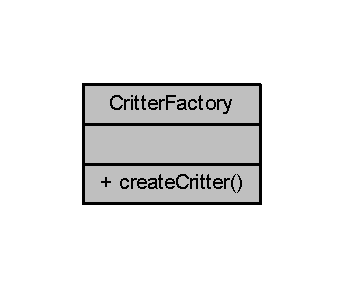
\includegraphics[width=165pt]{class_critter_factory__coll__graph}
\end{center}
\end{figure}
\subsection*{Public Types}
\begin{DoxyCompactItemize}
\item 
enum \hyperlink{class_critter_factory_a865a154e14b99d3dbf4d329a49210f6a}{Critter\+Type} \{ \hyperlink{class_critter_factory_a865a154e14b99d3dbf4d329a49210f6aaac2fdd0d6df8da9a2c6e984d010655c5}{C\+A\+T}, 
\hyperlink{class_critter_factory_a865a154e14b99d3dbf4d329a49210f6aaeecb28f72cdc5acb898c5a8256b05f29}{D\+O\+G}, 
\hyperlink{class_critter_factory_a865a154e14b99d3dbf4d329a49210f6aabb786a2c290b737c46c7be72df575d57}{W\+E\+R\+E\+C\+A\+T}, 
\hyperlink{class_critter_factory_a865a154e14b99d3dbf4d329a49210f6aa47578594f1bc7d73797a2a7fb0750aaf}{W\+E\+R\+E\+W\+O\+L\+F}
 \}
\end{DoxyCompactItemize}
\subsection*{Static Public Member Functions}
\begin{DoxyCompactItemize}
\item 
static \hyperlink{class_critter}{Critter} $\ast$ \hyperlink{class_critter_factory_a983fedc85e591f4b9fdebcf2b73853c8}{create\+Critter} (\hyperlink{class_critter_factory_a865a154e14b99d3dbf4d329a49210f6a}{Critter\+Type} type)
\begin{DoxyCompactList}\small\item\em Factory method for \hyperlink{class_critter}{Critter} class. \end{DoxyCompactList}\end{DoxyCompactItemize}


\subsection{Detailed Description}
Creates objects derived from \hyperlink{class_critter}{Critter}. Utility class that creates instance of a \hyperlink{class_critter}{Critter} subclass from a family of derived \hyperlink{class_critter}{Critter} classes. 

\subsection{Member Enumeration Documentation}
\hypertarget{class_critter_factory_a865a154e14b99d3dbf4d329a49210f6a}{\index{Critter\+Factory@{Critter\+Factory}!Critter\+Type@{Critter\+Type}}
\index{Critter\+Type@{Critter\+Type}!Critter\+Factory@{Critter\+Factory}}
\subsubsection[{Critter\+Type}]{\setlength{\rightskip}{0pt plus 5cm}enum {\bf Critter\+Factory\+::\+Critter\+Type}}}\label{class_critter_factory_a865a154e14b99d3dbf4d329a49210f6a}
\begin{Desc}
\item[Enumerator]\par
\begin{description}
\index{C\+A\+T@{C\+A\+T}!Critter\+Factory@{Critter\+Factory}}\index{Critter\+Factory@{Critter\+Factory}!C\+A\+T@{C\+A\+T}}\item[{\em 
\hypertarget{class_critter_factory_a865a154e14b99d3dbf4d329a49210f6aaac2fdd0d6df8da9a2c6e984d010655c5}{C\+A\+T}\label{class_critter_factory_a865a154e14b99d3dbf4d329a49210f6aaac2fdd0d6df8da9a2c6e984d010655c5}
}]\index{D\+O\+G@{D\+O\+G}!Critter\+Factory@{Critter\+Factory}}\index{Critter\+Factory@{Critter\+Factory}!D\+O\+G@{D\+O\+G}}\item[{\em 
\hypertarget{class_critter_factory_a865a154e14b99d3dbf4d329a49210f6aaeecb28f72cdc5acb898c5a8256b05f29}{D\+O\+G}\label{class_critter_factory_a865a154e14b99d3dbf4d329a49210f6aaeecb28f72cdc5acb898c5a8256b05f29}
}]\index{W\+E\+R\+E\+C\+A\+T@{W\+E\+R\+E\+C\+A\+T}!Critter\+Factory@{Critter\+Factory}}\index{Critter\+Factory@{Critter\+Factory}!W\+E\+R\+E\+C\+A\+T@{W\+E\+R\+E\+C\+A\+T}}\item[{\em 
\hypertarget{class_critter_factory_a865a154e14b99d3dbf4d329a49210f6aabb786a2c290b737c46c7be72df575d57}{W\+E\+R\+E\+C\+A\+T}\label{class_critter_factory_a865a154e14b99d3dbf4d329a49210f6aabb786a2c290b737c46c7be72df575d57}
}]\index{W\+E\+R\+E\+W\+O\+L\+F@{W\+E\+R\+E\+W\+O\+L\+F}!Critter\+Factory@{Critter\+Factory}}\index{Critter\+Factory@{Critter\+Factory}!W\+E\+R\+E\+W\+O\+L\+F@{W\+E\+R\+E\+W\+O\+L\+F}}\item[{\em 
\hypertarget{class_critter_factory_a865a154e14b99d3dbf4d329a49210f6aa47578594f1bc7d73797a2a7fb0750aaf}{W\+E\+R\+E\+W\+O\+L\+F}\label{class_critter_factory_a865a154e14b99d3dbf4d329a49210f6aa47578594f1bc7d73797a2a7fb0750aaf}
}]\end{description}
\end{Desc}


\subsection{Member Function Documentation}
\hypertarget{class_critter_factory_a983fedc85e591f4b9fdebcf2b73853c8}{\index{Critter\+Factory@{Critter\+Factory}!create\+Critter@{create\+Critter}}
\index{create\+Critter@{create\+Critter}!Critter\+Factory@{Critter\+Factory}}
\subsubsection[{create\+Critter}]{\setlength{\rightskip}{0pt plus 5cm}{\bf Critter} $\ast$ Critter\+Factory\+::create\+Critter (
\begin{DoxyParamCaption}
\item[{{\bf Critter\+Type}}]{type}
\end{DoxyParamCaption}
)\hspace{0.3cm}{\ttfamily [static]}}}\label{class_critter_factory_a983fedc85e591f4b9fdebcf2b73853c8}


Factory method for \hyperlink{class_critter}{Critter} class. 

\begin{DoxyReturn}{Returns}
\hyperlink{class_critter}{Critter} object (subclass of \hyperlink{class_critter}{Critter}).
\end{DoxyReturn}
The only method in \hyperlink{class_critter_factory}{Critter\+Factory}, \hyperlink{class_critter_factory_a983fedc85e591f4b9fdebcf2b73853c8}{create\+Critter()} cranks out \hyperlink{class_critter}{Critter} objects based on the enum parameter. 

Here is the caller graph for this function\+:
\nopagebreak
\begin{figure}[H]
\begin{center}
\leavevmode
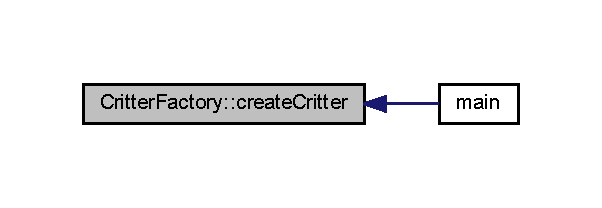
\includegraphics[width=289pt]{class_critter_factory_a983fedc85e591f4b9fdebcf2b73853c8_icgraph}
\end{center}
\end{figure}




The documentation for this class was generated from the following files\+:\begin{DoxyCompactItemize}
\item 
C\+O\+M\+P345/\+Assignment1\+\_\+no\+G\+U\+I/\+Critter\+Group\+Generator/\+Critter\+Group\+Generator/include/\hyperlink{_critter_factory_8h}{Critter\+Factory.\+h}\item 
C\+O\+M\+P345/\+Assignment1\+\_\+no\+G\+U\+I/\+Critter\+Group\+Generator/\+Critter\+Group\+Generator/src/game\+Objects/\hyperlink{_critter_factory_8cpp}{Critter\+Factory.\+cpp}\end{DoxyCompactItemize}

\hypertarget{class_critter_wave}{\section{Critter\+Wave Class Reference}
\label{class_critter_wave}\index{Critter\+Wave@{Critter\+Wave}}
}


Represents a wave of Critters. Class that has holds Critters in a map data structure, which represents a wave of Critters.  




{\ttfamily \#include $<$Critter\+Wave.\+h$>$}



Collaboration diagram for Critter\+Wave\+:
\nopagebreak
\begin{figure}[H]
\begin{center}
\leavevmode
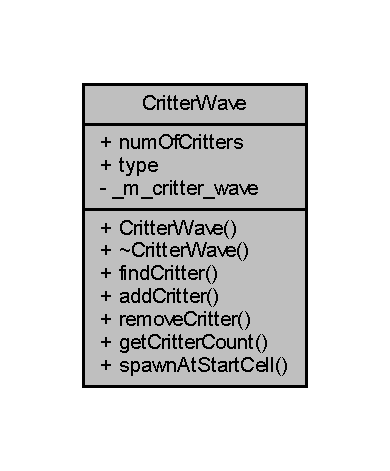
\includegraphics[width=187pt]{class_critter_wave__coll__graph}
\end{center}
\end{figure}
\subsection*{Classes}
\begin{DoxyCompactItemize}
\item 
struct \hyperlink{struct_critter_wave_1_1_critter_wave_deallocator}{Critter\+Wave\+Deallocator}
\begin{DoxyCompactList}\small\item\em Struct deallocating resources used in a \hyperlink{class_critter_wave}{Critter\+Wave} map. \end{DoxyCompactList}\end{DoxyCompactItemize}
\subsection*{Public Member Functions}
\begin{DoxyCompactItemize}
\item 
\hyperlink{class_critter_wave_a5c9542e09173535de5ce7fec7608eead}{Critter\+Wave} (int \hyperlink{class_critter_wave_a6c8edb08492ed068c5e4c5323695c29d}{num\+Of\+Critters}, \hyperlink{class_critter_factory_a865a154e14b99d3dbf4d329a49210f6a}{Critter\+Factory\+::\+Critter\+Type} \hyperlink{class_critter_wave_a15d8e4b3eb954f0dfa4f6224d90e0ae0}{type})
\begin{DoxyCompactList}\small\item\em This constructor sets the type and number of critters for the wave. \end{DoxyCompactList}\item 
\hyperlink{class_critter_wave_a89e6acba97071ff44a9493315a8f073b}{$\sim$\+Critter\+Wave} ()
\begin{DoxyCompactList}\small\item\em This destructor iterates through the map, calling a deallocator which deletes Critter$\ast$ references in a wave. \end{DoxyCompactList}\item 
\hyperlink{class_critter}{Critter} $\ast$ \hyperlink{class_critter_wave_a1244e59ebd702edd2530e6256779ace0}{find\+Critter} (int id) const 
\begin{DoxyCompactList}\small\item\em Returns a reference to a \hyperlink{class_critter}{Critter} in the map. \end{DoxyCompactList}\item 
void \hyperlink{class_critter_wave_a3c6dcf79b57cb7e208471c5bc387f22d}{add\+Critter} (int id, \hyperlink{class_critter}{Critter} $\ast$critter)
\begin{DoxyCompactList}\small\item\em Adding a \hyperlink{class_critter}{Critter} to the wave. \end{DoxyCompactList}\item 
void \hyperlink{class_critter_wave_aa7761b522b8774ef9b319861ae6ab844}{remove\+Critter} (int id)
\begin{DoxyCompactList}\small\item\em Remove a critter from the \hyperlink{class_critter_wave}{Critter\+Wave} map. \end{DoxyCompactList}\item 
int \hyperlink{class_critter_wave_a3c782475b9f1a73ddb658449592b8a33}{get\+Critter\+Count} () const 
\begin{DoxyCompactList}\small\item\em Returns how many critters are in a \hyperlink{class_critter_wave}{Critter\+Wave} map. \end{DoxyCompactList}\item 
void \hyperlink{class_critter_wave_a022f1d4bf44e35401a99e70ccd31dd87}{spawn\+At\+Start\+Cell} (int critter\+\_\+id, int row, int col)
\begin{DoxyCompactList}\small\item\em Set starting position of Critters in wave. \end{DoxyCompactList}\end{DoxyCompactItemize}
\subsection*{Public Attributes}
\begin{DoxyCompactItemize}
\item 
const int \hyperlink{class_critter_wave_a6c8edb08492ed068c5e4c5323695c29d}{num\+Of\+Critters}
\begin{DoxyCompactList}\small\item\em \hyperlink{class_map}{Map} representing a critter wave. \end{DoxyCompactList}\item 
\hyperlink{class_critter_factory_a865a154e14b99d3dbf4d329a49210f6a}{Critter\+Factory\+::\+Critter\+Type} \hyperlink{class_critter_wave_a15d8e4b3eb954f0dfa4f6224d90e0ae0}{type}
\begin{DoxyCompactList}\small\item\em Type of critter in a critter wave. \end{DoxyCompactList}\end{DoxyCompactItemize}
\subsection*{Private Attributes}
\begin{DoxyCompactItemize}
\item 
std\+::map$<$ int, \hyperlink{class_critter}{Critter} $\ast$ $>$ \hyperlink{class_critter_wave_a82475869f718062181e545afb8277217}{\+\_\+m\+\_\+critter\+\_\+wave}
\begin{DoxyCompactList}\small\item\em \hyperlink{class_map}{Map} representing a critter wave. \end{DoxyCompactList}\end{DoxyCompactItemize}
\subsection*{Friends}
\begin{DoxyCompactItemize}
\item 
std\+::ostream \& \hyperlink{class_critter_wave_a06016c30b019307c3fd6e11c447ffbe0}{operator$<$$<$} (std\+::ostream \&output, const \hyperlink{class_critter_wave}{Critter\+Wave} \&critter\+\_\+wave)
\begin{DoxyCompactList}\small\item\em Overloaded cout operator to print out Critter\+Waves. \end{DoxyCompactList}\end{DoxyCompactItemize}


\subsection{Detailed Description}
Represents a wave of Critters. Class that has holds Critters in a map data structure, which represents a wave of Critters. 

\subsection{Constructor \& Destructor Documentation}
\hypertarget{class_critter_wave_a5c9542e09173535de5ce7fec7608eead}{\index{Critter\+Wave@{Critter\+Wave}!Critter\+Wave@{Critter\+Wave}}
\index{Critter\+Wave@{Critter\+Wave}!Critter\+Wave@{Critter\+Wave}}
\subsubsection[{Critter\+Wave}]{\setlength{\rightskip}{0pt plus 5cm}Critter\+Wave\+::\+Critter\+Wave (
\begin{DoxyParamCaption}
\item[{int}]{num\+Of\+Critters, }
\item[{{\bf Critter\+Factory\+::\+Critter\+Type}}]{type}
\end{DoxyParamCaption}
)}}\label{class_critter_wave_a5c9542e09173535de5ce7fec7608eead}


This constructor sets the type and number of critters for the wave. 

\hypertarget{class_critter_wave_a89e6acba97071ff44a9493315a8f073b}{\index{Critter\+Wave@{Critter\+Wave}!````~Critter\+Wave@{$\sim$\+Critter\+Wave}}
\index{````~Critter\+Wave@{$\sim$\+Critter\+Wave}!Critter\+Wave@{Critter\+Wave}}
\subsubsection[{$\sim$\+Critter\+Wave}]{\setlength{\rightskip}{0pt plus 5cm}Critter\+Wave\+::$\sim$\+Critter\+Wave (
\begin{DoxyParamCaption}
{}
\end{DoxyParamCaption}
)}}\label{class_critter_wave_a89e6acba97071ff44a9493315a8f073b}


This destructor iterates through the map, calling a deallocator which deletes Critter$\ast$ references in a wave. 



\subsection{Member Function Documentation}
\hypertarget{class_critter_wave_a3c6dcf79b57cb7e208471c5bc387f22d}{\index{Critter\+Wave@{Critter\+Wave}!add\+Critter@{add\+Critter}}
\index{add\+Critter@{add\+Critter}!Critter\+Wave@{Critter\+Wave}}
\subsubsection[{add\+Critter}]{\setlength{\rightskip}{0pt plus 5cm}void Critter\+Wave\+::add\+Critter (
\begin{DoxyParamCaption}
\item[{int}]{id, }
\item[{{\bf Critter} $\ast$}]{critter}
\end{DoxyParamCaption}
)}}\label{class_critter_wave_a3c6dcf79b57cb7e208471c5bc387f22d}


Adding a \hyperlink{class_critter}{Critter} to the wave. 



Here is the caller graph for this function\+:
\nopagebreak
\begin{figure}[H]
\begin{center}
\leavevmode
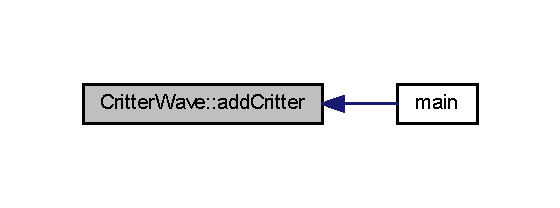
\includegraphics[width=269pt]{class_critter_wave_a3c6dcf79b57cb7e208471c5bc387f22d_icgraph}
\end{center}
\end{figure}


\hypertarget{class_critter_wave_a1244e59ebd702edd2530e6256779ace0}{\index{Critter\+Wave@{Critter\+Wave}!find\+Critter@{find\+Critter}}
\index{find\+Critter@{find\+Critter}!Critter\+Wave@{Critter\+Wave}}
\subsubsection[{find\+Critter}]{\setlength{\rightskip}{0pt plus 5cm}{\bf Critter} $\ast$ Critter\+Wave\+::find\+Critter (
\begin{DoxyParamCaption}
\item[{int}]{id}
\end{DoxyParamCaption}
) const}}\label{class_critter_wave_a1244e59ebd702edd2530e6256779ace0}


Returns a reference to a \hyperlink{class_critter}{Critter} in the map. 


\begin{DoxyParams}{Parameters}
{\em critter\+\_\+id} & Id of the \hyperlink{class_critter}{Critter} to be found \\
\hline
\end{DoxyParams}
\begin{DoxyReturn}{Returns}
Pointer to a \hyperlink{class_critter}{Critter} in the map.
\end{DoxyReturn}
Iterate through the map, looking for the given \hyperlink{class_critter}{Critter} id. If end of map is reached, return null, else return the Critter$\ast$. 

Here is the caller graph for this function\+:
\nopagebreak
\begin{figure}[H]
\begin{center}
\leavevmode
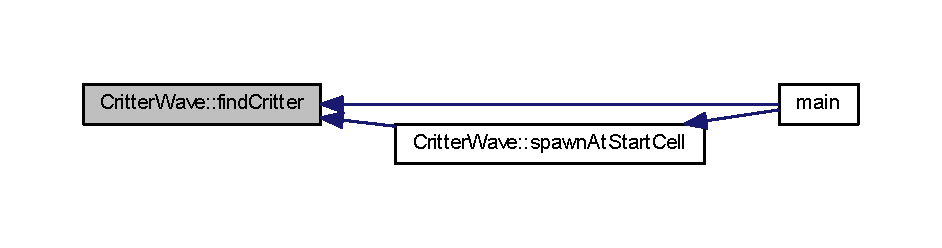
\includegraphics[width=350pt]{class_critter_wave_a1244e59ebd702edd2530e6256779ace0_icgraph}
\end{center}
\end{figure}


\hypertarget{class_critter_wave_a3c782475b9f1a73ddb658449592b8a33}{\index{Critter\+Wave@{Critter\+Wave}!get\+Critter\+Count@{get\+Critter\+Count}}
\index{get\+Critter\+Count@{get\+Critter\+Count}!Critter\+Wave@{Critter\+Wave}}
\subsubsection[{get\+Critter\+Count}]{\setlength{\rightskip}{0pt plus 5cm}int Critter\+Wave\+::get\+Critter\+Count (
\begin{DoxyParamCaption}
{}
\end{DoxyParamCaption}
) const}}\label{class_critter_wave_a3c782475b9f1a73ddb658449592b8a33}


Returns how many critters are in a \hyperlink{class_critter_wave}{Critter\+Wave} map. 

\begin{DoxyReturn}{Returns}
Count of number of Critters in a wave. 
\end{DoxyReturn}
\hypertarget{class_critter_wave_aa7761b522b8774ef9b319861ae6ab844}{\index{Critter\+Wave@{Critter\+Wave}!remove\+Critter@{remove\+Critter}}
\index{remove\+Critter@{remove\+Critter}!Critter\+Wave@{Critter\+Wave}}
\subsubsection[{remove\+Critter}]{\setlength{\rightskip}{0pt plus 5cm}void Critter\+Wave\+::remove\+Critter (
\begin{DoxyParamCaption}
\item[{int}]{id}
\end{DoxyParamCaption}
)}}\label{class_critter_wave_aa7761b522b8774ef9b319861ae6ab844}


Remove a critter from the \hyperlink{class_critter_wave}{Critter\+Wave} map. 


\begin{DoxyParams}{Parameters}
{\em critter\+\_\+id} & Id of the \hyperlink{class_critter}{Critter} to be removed\\
\hline
\end{DoxyParams}
Iterate through the map, looking for the given \hyperlink{class_critter}{Critter} id, if found, delete the pointer and remove the Critter$\ast$ from the map. 

Here is the caller graph for this function\+:
\nopagebreak
\begin{figure}[H]
\begin{center}
\leavevmode
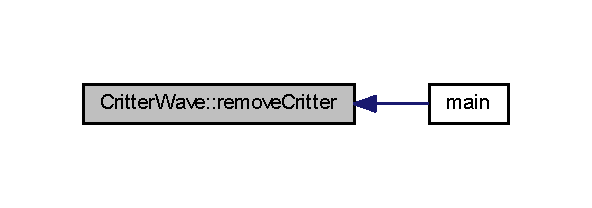
\includegraphics[width=284pt]{class_critter_wave_aa7761b522b8774ef9b319861ae6ab844_icgraph}
\end{center}
\end{figure}


\hypertarget{class_critter_wave_a022f1d4bf44e35401a99e70ccd31dd87}{\index{Critter\+Wave@{Critter\+Wave}!spawn\+At\+Start\+Cell@{spawn\+At\+Start\+Cell}}
\index{spawn\+At\+Start\+Cell@{spawn\+At\+Start\+Cell}!Critter\+Wave@{Critter\+Wave}}
\subsubsection[{spawn\+At\+Start\+Cell}]{\setlength{\rightskip}{0pt plus 5cm}void Critter\+Wave\+::spawn\+At\+Start\+Cell (
\begin{DoxyParamCaption}
\item[{int}]{critter\+\_\+id, }
\item[{int}]{row, }
\item[{int}]{col}
\end{DoxyParamCaption}
)}}\label{class_critter_wave_a022f1d4bf44e35401a99e70ccd31dd87}


Set starting position of Critters in wave. 

\begin{DoxyReturn}{Returns}
Void. 
\end{DoxyReturn}


Here is the call graph for this function\+:
\nopagebreak
\begin{figure}[H]
\begin{center}
\leavevmode
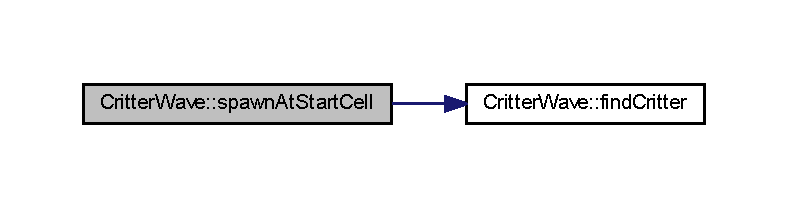
\includegraphics[width=350pt]{class_critter_wave_a022f1d4bf44e35401a99e70ccd31dd87_cgraph}
\end{center}
\end{figure}




Here is the caller graph for this function\+:
\nopagebreak
\begin{figure}[H]
\begin{center}
\leavevmode
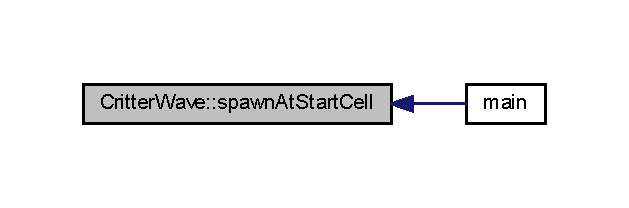
\includegraphics[width=302pt]{class_critter_wave_a022f1d4bf44e35401a99e70ccd31dd87_icgraph}
\end{center}
\end{figure}




\subsection{Friends And Related Function Documentation}
\hypertarget{class_critter_wave_a06016c30b019307c3fd6e11c447ffbe0}{\index{Critter\+Wave@{Critter\+Wave}!operator$<$$<$@{operator$<$$<$}}
\index{operator$<$$<$@{operator$<$$<$}!Critter\+Wave@{Critter\+Wave}}
\subsubsection[{operator$<$$<$}]{\setlength{\rightskip}{0pt plus 5cm}std\+::ostream\& operator$<$$<$ (
\begin{DoxyParamCaption}
\item[{std\+::ostream \&}]{output, }
\item[{const {\bf Critter\+Wave} \&}]{critter\+\_\+wave}
\end{DoxyParamCaption}
)\hspace{0.3cm}{\ttfamily [friend]}}}\label{class_critter_wave_a06016c30b019307c3fd6e11c447ffbe0}


Overloaded cout operator to print out Critter\+Waves. 


\begin{DoxyParams}{Parameters}
{\em output} & Output stream address \\
\hline
{\em critter} & Const address to \hyperlink{class_critter_wave}{Critter\+Wave} \\
\hline
\end{DoxyParams}
\begin{DoxyReturn}{Returns}
Address to output stream 
\end{DoxyReturn}


\subsection{Member Data Documentation}
\hypertarget{class_critter_wave_a82475869f718062181e545afb8277217}{\index{Critter\+Wave@{Critter\+Wave}!\+\_\+m\+\_\+critter\+\_\+wave@{\+\_\+m\+\_\+critter\+\_\+wave}}
\index{\+\_\+m\+\_\+critter\+\_\+wave@{\+\_\+m\+\_\+critter\+\_\+wave}!Critter\+Wave@{Critter\+Wave}}
\subsubsection[{\+\_\+m\+\_\+critter\+\_\+wave}]{\setlength{\rightskip}{0pt plus 5cm}std\+::map$<$int, {\bf Critter}$\ast$$>$ Critter\+Wave\+::\+\_\+m\+\_\+critter\+\_\+wave\hspace{0.3cm}{\ttfamily [private]}}}\label{class_critter_wave_a82475869f718062181e545afb8277217}


\hyperlink{class_map}{Map} representing a critter wave. 

\hypertarget{class_critter_wave_a6c8edb08492ed068c5e4c5323695c29d}{\index{Critter\+Wave@{Critter\+Wave}!num\+Of\+Critters@{num\+Of\+Critters}}
\index{num\+Of\+Critters@{num\+Of\+Critters}!Critter\+Wave@{Critter\+Wave}}
\subsubsection[{num\+Of\+Critters}]{\setlength{\rightskip}{0pt plus 5cm}const int Critter\+Wave\+::num\+Of\+Critters}}\label{class_critter_wave_a6c8edb08492ed068c5e4c5323695c29d}


\hyperlink{class_map}{Map} representing a critter wave. 

\hypertarget{class_critter_wave_a15d8e4b3eb954f0dfa4f6224d90e0ae0}{\index{Critter\+Wave@{Critter\+Wave}!type@{type}}
\index{type@{type}!Critter\+Wave@{Critter\+Wave}}
\subsubsection[{type}]{\setlength{\rightskip}{0pt plus 5cm}{\bf Critter\+Factory\+::\+Critter\+Type} Critter\+Wave\+::type}}\label{class_critter_wave_a15d8e4b3eb954f0dfa4f6224d90e0ae0}


Type of critter in a critter wave. 



The documentation for this class was generated from the following files\+:\begin{DoxyCompactItemize}
\item 
C\+O\+M\+P345/\+Assignment1\+\_\+no\+G\+U\+I/\+Critter\+Group\+Generator/\+Critter\+Group\+Generator/include/\hyperlink{_critter_wave_8h}{Critter\+Wave.\+h}\item 
C\+O\+M\+P345/\+Assignment1\+\_\+no\+G\+U\+I/\+Critter\+Group\+Generator/\+Critter\+Group\+Generator/src/game\+Objects/\hyperlink{_critter_wave_8cpp}{Critter\+Wave.\+cpp}\end{DoxyCompactItemize}

\hypertarget{struct_critter_wave_1_1_critter_wave_deallocator}{\section{Critter\+Wave\+:\+:Critter\+Wave\+Deallocator Struct Reference}
\label{struct_critter_wave_1_1_critter_wave_deallocator}\index{Critter\+Wave\+::\+Critter\+Wave\+Deallocator@{Critter\+Wave\+::\+Critter\+Wave\+Deallocator}}
}


Struct deallocating resources used in a \hyperlink{class_critter_wave}{Critter\+Wave} map.  




Collaboration diagram for Critter\+Wave\+:\+:Critter\+Wave\+Deallocator\+:
\nopagebreak
\begin{figure}[H]
\begin{center}
\leavevmode
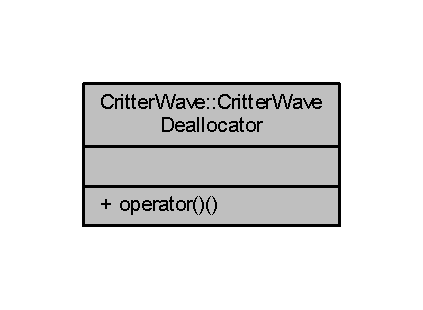
\includegraphics[width=203pt]{struct_critter_wave_1_1_critter_wave_deallocator__coll__graph}
\end{center}
\end{figure}
\subsection*{Public Member Functions}
\begin{DoxyCompactItemize}
\item 
void \hyperlink{struct_critter_wave_1_1_critter_wave_deallocator_a3b5befe161e66cd3d7cf9d72b948cd6a}{operator()} (const std\+::pair$<$ int, \hyperlink{class_critter}{Critter} $\ast$ $>$ \&item)
\begin{DoxyCompactList}\small\item\em Overloading of the function operator () \end{DoxyCompactList}\end{DoxyCompactItemize}


\subsection{Detailed Description}
Struct deallocating resources used in a \hyperlink{class_critter_wave}{Critter\+Wave} map. 

\subsection{Member Function Documentation}
\hypertarget{struct_critter_wave_1_1_critter_wave_deallocator_a3b5befe161e66cd3d7cf9d72b948cd6a}{\index{Critter\+Wave\+::\+Critter\+Wave\+Deallocator@{Critter\+Wave\+::\+Critter\+Wave\+Deallocator}!operator()@{operator()}}
\index{operator()@{operator()}!Critter\+Wave\+::\+Critter\+Wave\+Deallocator@{Critter\+Wave\+::\+Critter\+Wave\+Deallocator}}
\subsubsection[{operator()}]{\setlength{\rightskip}{0pt plus 5cm}void Critter\+Wave\+::\+Critter\+Wave\+Deallocator\+::operator() (
\begin{DoxyParamCaption}
\item[{const std\+::pair$<$ int, {\bf Critter} $\ast$ $>$ \&}]{item}
\end{DoxyParamCaption}
)\hspace{0.3cm}{\ttfamily [inline]}}}\label{struct_critter_wave_1_1_critter_wave_deallocator_a3b5befe161e66cd3d7cf9d72b948cd6a}


Overloading of the function operator () 


\begin{DoxyParams}{Parameters}
{\em item} & Coupled values that represents an item in the map \\
\hline
\end{DoxyParams}
\begin{DoxyReturn}{Returns}
Void. 
\end{DoxyReturn}


The documentation for this struct was generated from the following file\+:\begin{DoxyCompactItemize}
\item 
C\+O\+M\+P345/\+Assignment1\+\_\+no\+G\+U\+I/\+Critter\+Group\+Generator/\+Critter\+Group\+Generator/include/\hyperlink{_critter_wave_8h}{Critter\+Wave.\+h}\end{DoxyCompactItemize}

\hypertarget{class_dog}{\section{Dog Class Reference}
\label{class_dog}\index{Dog@{Dog}}
}


Class for \hyperlink{class_dog}{Dog}. Subclass of \hyperlink{class_critter}{Critter}.  




{\ttfamily \#include $<$Dog.\+h$>$}



Inheritance diagram for Dog\+:
\nopagebreak
\begin{figure}[H]
\begin{center}
\leavevmode
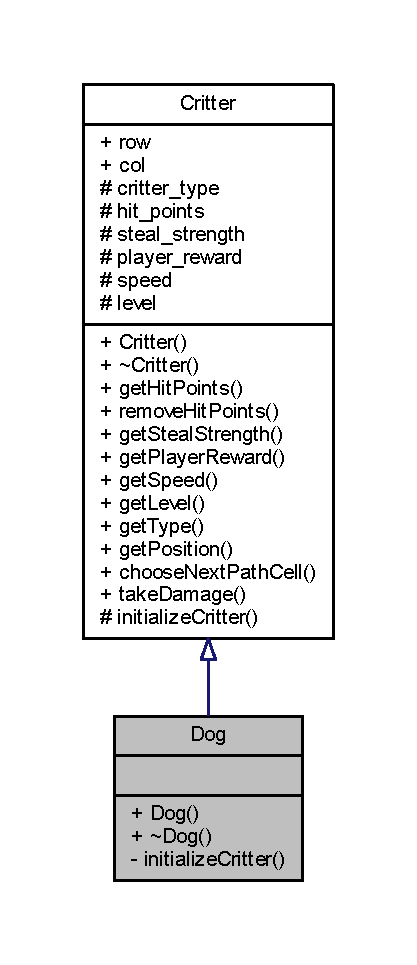
\includegraphics[width=200pt]{class_dog__inherit__graph}
\end{center}
\end{figure}


Collaboration diagram for Dog\+:
\nopagebreak
\begin{figure}[H]
\begin{center}
\leavevmode
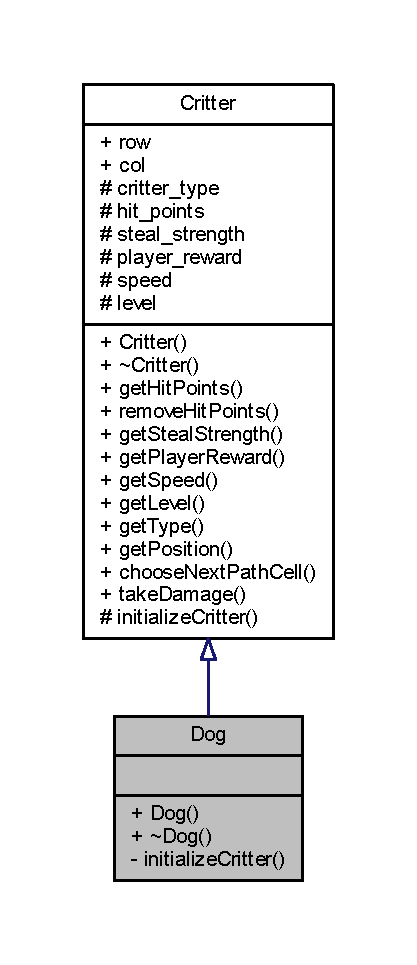
\includegraphics[width=200pt]{class_dog__coll__graph}
\end{center}
\end{figure}
\subsection*{Public Member Functions}
\begin{DoxyCompactItemize}
\item 
\hyperlink{class_dog_a16e01978bb90b2989ee3da3e87071b1b}{Dog} ()
\begin{DoxyCompactList}\small\item\em The \hyperlink{class_dog}{Dog} constructor. Calls \hyperlink{class_dog_ab512ed7b74de6ab907e4199f98d82566}{initialize\+Critter()} to set attributes of the \hyperlink{class_dog}{Dog} object. \end{DoxyCompactList}\item 
\hyperlink{class_dog_aeacf410641eab28eabea6bc5269eb4ef}{$\sim$\+Dog} ()
\end{DoxyCompactItemize}
\subsection*{Private Member Functions}
\begin{DoxyCompactItemize}
\item 
virtual void \hyperlink{class_dog_ab512ed7b74de6ab907e4199f98d82566}{initialize\+Critter} ()
\begin{DoxyCompactList}\small\item\em Initialization function for a \hyperlink{class_dog}{Dog}. \end{DoxyCompactList}\end{DoxyCompactItemize}
\subsection*{Additional Inherited Members}


\subsection{Detailed Description}
Class for \hyperlink{class_dog}{Dog}. Subclass of \hyperlink{class_critter}{Critter}. 

\subsection{Constructor \& Destructor Documentation}
\hypertarget{class_dog_a16e01978bb90b2989ee3da3e87071b1b}{\index{Dog@{Dog}!Dog@{Dog}}
\index{Dog@{Dog}!Dog@{Dog}}
\subsubsection[{Dog}]{\setlength{\rightskip}{0pt plus 5cm}Dog\+::\+Dog (
\begin{DoxyParamCaption}
{}
\end{DoxyParamCaption}
)}}\label{class_dog_a16e01978bb90b2989ee3da3e87071b1b}


The \hyperlink{class_dog}{Dog} constructor. Calls \hyperlink{class_dog_ab512ed7b74de6ab907e4199f98d82566}{initialize\+Critter()} to set attributes of the \hyperlink{class_dog}{Dog} object. 



Here is the call graph for this function\+:
\nopagebreak
\begin{figure}[H]
\begin{center}
\leavevmode
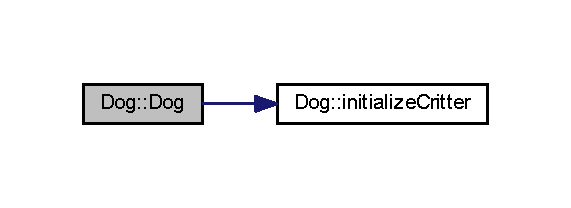
\includegraphics[width=274pt]{class_dog_a16e01978bb90b2989ee3da3e87071b1b_cgraph}
\end{center}
\end{figure}


\hypertarget{class_dog_aeacf410641eab28eabea6bc5269eb4ef}{\index{Dog@{Dog}!````~Dog@{$\sim$\+Dog}}
\index{````~Dog@{$\sim$\+Dog}!Dog@{Dog}}
\subsubsection[{$\sim$\+Dog}]{\setlength{\rightskip}{0pt plus 5cm}Dog\+::$\sim$\+Dog (
\begin{DoxyParamCaption}
{}
\end{DoxyParamCaption}
)\hspace{0.3cm}{\ttfamily [inline]}}}\label{class_dog_aeacf410641eab28eabea6bc5269eb4ef}


\subsection{Member Function Documentation}
\hypertarget{class_dog_ab512ed7b74de6ab907e4199f98d82566}{\index{Dog@{Dog}!initialize\+Critter@{initialize\+Critter}}
\index{initialize\+Critter@{initialize\+Critter}!Dog@{Dog}}
\subsubsection[{initialize\+Critter}]{\setlength{\rightskip}{0pt plus 5cm}void Dog\+::initialize\+Critter (
\begin{DoxyParamCaption}
{}
\end{DoxyParamCaption}
)\hspace{0.3cm}{\ttfamily [private]}, {\ttfamily [virtual]}}}\label{class_dog_ab512ed7b74de6ab907e4199f98d82566}


Initialization function for a \hyperlink{class_dog}{Dog}. 

\begin{DoxyReturn}{Returns}
Void.
\end{DoxyReturn}
Initialization specific to a \hyperlink{class_cat}{Cat} object 

Implements \hyperlink{class_critter_ab903f6d28ef3fc70808390fef8816b79}{Critter}.



Here is the caller graph for this function\+:
\nopagebreak
\begin{figure}[H]
\begin{center}
\leavevmode
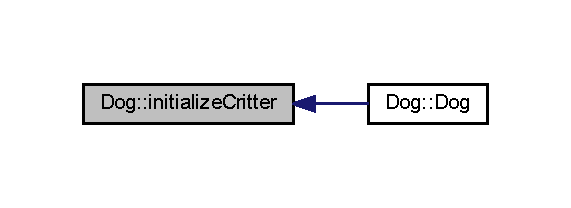
\includegraphics[width=274pt]{class_dog_ab512ed7b74de6ab907e4199f98d82566_icgraph}
\end{center}
\end{figure}




The documentation for this class was generated from the following files\+:\begin{DoxyCompactItemize}
\item 
C\+O\+M\+P345/\+Assignment1\+\_\+no\+G\+U\+I/\+Critter\+Group\+Generator/\+Critter\+Group\+Generator/include/\hyperlink{_dog_8h}{Dog.\+h}\item 
C\+O\+M\+P345/\+Assignment1\+\_\+no\+G\+U\+I/\+Critter\+Group\+Generator/\+Critter\+Group\+Generator/src/game\+Objects/\hyperlink{_dog_8cpp}{Dog.\+cpp}\end{DoxyCompactItemize}

\hypertarget{struct_map_1_1_exit_cell}{\section{Map\+:\+:Exit\+Cell Struct Reference}
\label{struct_map_1_1_exit_cell}\index{Map\+::\+Exit\+Cell@{Map\+::\+Exit\+Cell}}
}


Derived from base struct \hyperlink{struct_map_1_1_cell}{Cell}.  




{\ttfamily \#include $<$Map.\+h$>$}



Inheritance diagram for Map\+:\+:Exit\+Cell\+:
\nopagebreak
\begin{figure}[H]
\begin{center}
\leavevmode
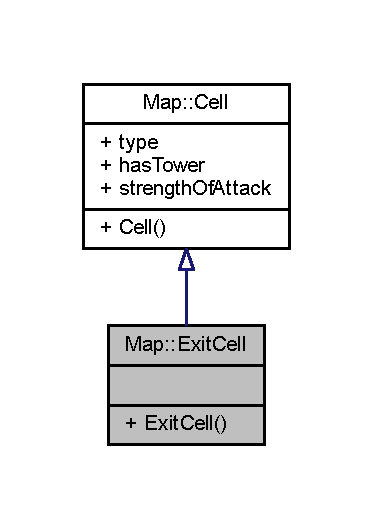
\includegraphics[width=179pt]{struct_map_1_1_exit_cell__inherit__graph}
\end{center}
\end{figure}


Collaboration diagram for Map\+:\+:Exit\+Cell\+:
\nopagebreak
\begin{figure}[H]
\begin{center}
\leavevmode
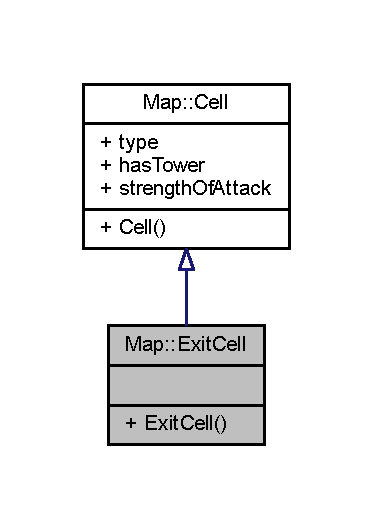
\includegraphics[width=179pt]{struct_map_1_1_exit_cell__coll__graph}
\end{center}
\end{figure}
\subsection*{Public Member Functions}
\begin{DoxyCompactItemize}
\item 
\hyperlink{struct_map_1_1_exit_cell_a86f2e252462c87d45cb9a8b513e8bed1}{Exit\+Cell} ()
\end{DoxyCompactItemize}
\subsection*{Additional Inherited Members}


\subsection{Detailed Description}
Derived from base struct \hyperlink{struct_map_1_1_cell}{Cell}. 

\subsection{Constructor \& Destructor Documentation}
\hypertarget{struct_map_1_1_exit_cell_a86f2e252462c87d45cb9a8b513e8bed1}{\index{Map\+::\+Exit\+Cell@{Map\+::\+Exit\+Cell}!Exit\+Cell@{Exit\+Cell}}
\index{Exit\+Cell@{Exit\+Cell}!Map\+::\+Exit\+Cell@{Map\+::\+Exit\+Cell}}
\subsubsection[{Exit\+Cell}]{\setlength{\rightskip}{0pt plus 5cm}Map\+::\+Exit\+Cell\+::\+Exit\+Cell (
\begin{DoxyParamCaption}
{}
\end{DoxyParamCaption}
)\hspace{0.3cm}{\ttfamily [inline]}}}\label{struct_map_1_1_exit_cell_a86f2e252462c87d45cb9a8b513e8bed1}


The documentation for this struct was generated from the following file\+:\begin{DoxyCompactItemize}
\item 
C\+O\+M\+P345/\+Assignment1\+\_\+no\+G\+U\+I/\+Critter\+Group\+Generator/\+Critter\+Group\+Generator/include/\hyperlink{_map_8h}{Map.\+h}\end{DoxyCompactItemize}

\hypertarget{class_map}{\section{Map Class Reference}
\label{class_map}\index{Map@{Map}}
}


Class for \hyperlink{class_map}{Map}. Stub class of map for Critters.  




{\ttfamily \#include $<$Map.\+h$>$}



Collaboration diagram for Map\+:
\nopagebreak
\begin{figure}[H]
\begin{center}
\leavevmode
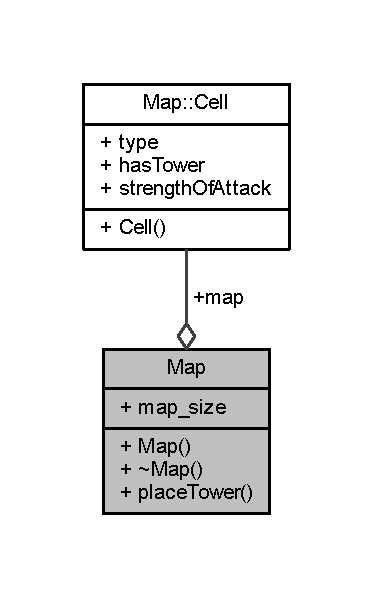
\includegraphics[width=179pt]{class_map__coll__graph}
\end{center}
\end{figure}
\subsection*{Classes}
\begin{DoxyCompactItemize}
\item 
struct \hyperlink{struct_map_1_1_cell}{Cell}
\begin{DoxyCompactList}\small\item\em Base struct for \hyperlink{struct_map_1_1_cell}{Cell} objects in a \hyperlink{class_map}{Map}. \end{DoxyCompactList}\item 
struct \hyperlink{struct_map_1_1_exit_cell}{Exit\+Cell}
\begin{DoxyCompactList}\small\item\em Derived from base struct \hyperlink{struct_map_1_1_cell}{Cell}. \end{DoxyCompactList}\item 
struct \hyperlink{struct_map_1_1_path_cell}{Path\+Cell}
\begin{DoxyCompactList}\small\item\em Derived from base struct \hyperlink{struct_map_1_1_cell}{Cell}. \end{DoxyCompactList}\item 
struct \hyperlink{struct_map_1_1_scenery_cell}{Scenery\+Cell}
\begin{DoxyCompactList}\small\item\em Derived from base struct \hyperlink{struct_map_1_1_cell}{Cell}. \end{DoxyCompactList}\item 
struct \hyperlink{struct_map_1_1_start_cell}{Start\+Cell}
\begin{DoxyCompactList}\small\item\em Derived from base struct \hyperlink{struct_map_1_1_cell}{Cell}. \end{DoxyCompactList}\item 
struct \hyperlink{struct_map_1_1_tower_cell}{Tower\+Cell}
\begin{DoxyCompactList}\small\item\em Derived from base struct \hyperlink{struct_map_1_1_cell}{Cell}. \end{DoxyCompactList}\end{DoxyCompactItemize}
\subsection*{Public Types}
\begin{DoxyCompactItemize}
\item 
enum \hyperlink{class_map_a25b1781a19b5a600a92f0487b823b272}{Cell\+Type} \{ \\*
\hyperlink{class_map_a25b1781a19b5a600a92f0487b823b272a887dcf135465781cd226cb80beeed332}{S\+C\+E\+N\+E\+R\+Y}, 
\hyperlink{class_map_a25b1781a19b5a600a92f0487b823b272a85ec32a17e33d95e9196319cd62060b3}{P\+A\+T\+H}, 
\hyperlink{class_map_a25b1781a19b5a600a92f0487b823b272a6a7572793842e84c9a4e94cfa9e417bb}{S\+T\+A\+R\+T}, 
\hyperlink{class_map_a25b1781a19b5a600a92f0487b823b272a0947300fe39206c7e2f5174d50974ba0}{E\+X\+I\+T}, 
\\*
\hyperlink{class_map_a25b1781a19b5a600a92f0487b823b272a80b3934f045ce22b4394dbb4e55c5645}{T\+O\+W\+E\+R}
 \}
\end{DoxyCompactItemize}
\subsection*{Public Member Functions}
\begin{DoxyCompactItemize}
\item 
\hyperlink{class_map_a0f5ad0fd4563497b4214038cbca8b582}{Map} ()
\item 
\hyperlink{class_map_aa403fbe09394ccf39747588f5168e3b2}{$\sim$\+Map} ()
\item 
void \hyperlink{class_map_a0a7e6088ebbdc4fa9b82896841933014}{place\+Tower} (int row, int col)
\begin{DoxyCompactList}\small\item\em Set a scenery cell to a tower cell. \end{DoxyCompactList}\end{DoxyCompactItemize}
\subsection*{Public Attributes}
\begin{DoxyCompactItemize}
\item 
\hyperlink{struct_map_1_1_cell}{Map\+::\+Cell} \hyperlink{class_map_aa5d63b554ad19c18cdc9911536e42001}{map} \mbox{[}\hyperlink{class_map_a6f922edb15340e98aee860d269e50703}{map\+\_\+size}\mbox{]}\mbox{[}\hyperlink{class_map_a6f922edb15340e98aee860d269e50703}{map\+\_\+size}\mbox{]}
\begin{DoxyCompactList}\small\item\em 2\+D array representing the map grid. \end{DoxyCompactList}\end{DoxyCompactItemize}
\subsection*{Static Public Attributes}
\begin{DoxyCompactItemize}
\item 
static const int \hyperlink{class_map_a6f922edb15340e98aee860d269e50703}{map\+\_\+size} = 5
\end{DoxyCompactItemize}
\subsection*{Friends}
\begin{DoxyCompactItemize}
\item 
std\+::ostream \& \hyperlink{class_map_aebdb7e7ad7d1b28f8e1b3a0b0917bb9c}{operator$<$$<$} (std\+::ostream \&output, const \hyperlink{class_map}{Map} \&\hyperlink{class_map_aa5d63b554ad19c18cdc9911536e42001}{map})
\begin{DoxyCompactList}\small\item\em Overloaded cout operator to print out Maps. \end{DoxyCompactList}\end{DoxyCompactItemize}


\subsection{Detailed Description}
Class for \hyperlink{class_map}{Map}. Stub class of map for Critters. 

\subsection{Member Enumeration Documentation}
\hypertarget{class_map_a25b1781a19b5a600a92f0487b823b272}{\index{Map@{Map}!Cell\+Type@{Cell\+Type}}
\index{Cell\+Type@{Cell\+Type}!Map@{Map}}
\subsubsection[{Cell\+Type}]{\setlength{\rightskip}{0pt plus 5cm}enum {\bf Map\+::\+Cell\+Type}}}\label{class_map_a25b1781a19b5a600a92f0487b823b272}
\begin{Desc}
\item[Enumerator]\par
\begin{description}
\index{S\+C\+E\+N\+E\+R\+Y@{S\+C\+E\+N\+E\+R\+Y}!Map@{Map}}\index{Map@{Map}!S\+C\+E\+N\+E\+R\+Y@{S\+C\+E\+N\+E\+R\+Y}}\item[{\em 
\hypertarget{class_map_a25b1781a19b5a600a92f0487b823b272a887dcf135465781cd226cb80beeed332}{S\+C\+E\+N\+E\+R\+Y}\label{class_map_a25b1781a19b5a600a92f0487b823b272a887dcf135465781cd226cb80beeed332}
}]\index{P\+A\+T\+H@{P\+A\+T\+H}!Map@{Map}}\index{Map@{Map}!P\+A\+T\+H@{P\+A\+T\+H}}\item[{\em 
\hypertarget{class_map_a25b1781a19b5a600a92f0487b823b272a85ec32a17e33d95e9196319cd62060b3}{P\+A\+T\+H}\label{class_map_a25b1781a19b5a600a92f0487b823b272a85ec32a17e33d95e9196319cd62060b3}
}]\index{S\+T\+A\+R\+T@{S\+T\+A\+R\+T}!Map@{Map}}\index{Map@{Map}!S\+T\+A\+R\+T@{S\+T\+A\+R\+T}}\item[{\em 
\hypertarget{class_map_a25b1781a19b5a600a92f0487b823b272a6a7572793842e84c9a4e94cfa9e417bb}{S\+T\+A\+R\+T}\label{class_map_a25b1781a19b5a600a92f0487b823b272a6a7572793842e84c9a4e94cfa9e417bb}
}]\index{E\+X\+I\+T@{E\+X\+I\+T}!Map@{Map}}\index{Map@{Map}!E\+X\+I\+T@{E\+X\+I\+T}}\item[{\em 
\hypertarget{class_map_a25b1781a19b5a600a92f0487b823b272a0947300fe39206c7e2f5174d50974ba0}{E\+X\+I\+T}\label{class_map_a25b1781a19b5a600a92f0487b823b272a0947300fe39206c7e2f5174d50974ba0}
}]\index{T\+O\+W\+E\+R@{T\+O\+W\+E\+R}!Map@{Map}}\index{Map@{Map}!T\+O\+W\+E\+R@{T\+O\+W\+E\+R}}\item[{\em 
\hypertarget{class_map_a25b1781a19b5a600a92f0487b823b272a80b3934f045ce22b4394dbb4e55c5645}{T\+O\+W\+E\+R}\label{class_map_a25b1781a19b5a600a92f0487b823b272a80b3934f045ce22b4394dbb4e55c5645}
}]\end{description}
\end{Desc}


\subsection{Constructor \& Destructor Documentation}
\hypertarget{class_map_a0f5ad0fd4563497b4214038cbca8b582}{\index{Map@{Map}!Map@{Map}}
\index{Map@{Map}!Map@{Map}}
\subsubsection[{Map}]{\setlength{\rightskip}{0pt plus 5cm}Map\+::\+Map (
\begin{DoxyParamCaption}
{}
\end{DoxyParamCaption}
)\hspace{0.3cm}{\ttfamily [inline]}}}\label{class_map_a0f5ad0fd4563497b4214038cbca8b582}
\hypertarget{class_map_aa403fbe09394ccf39747588f5168e3b2}{\index{Map@{Map}!````~Map@{$\sim$\+Map}}
\index{````~Map@{$\sim$\+Map}!Map@{Map}}
\subsubsection[{$\sim$\+Map}]{\setlength{\rightskip}{0pt plus 5cm}Map\+::$\sim$\+Map (
\begin{DoxyParamCaption}
{}
\end{DoxyParamCaption}
)\hspace{0.3cm}{\ttfamily [inline]}}}\label{class_map_aa403fbe09394ccf39747588f5168e3b2}


\subsection{Member Function Documentation}
\hypertarget{class_map_a0a7e6088ebbdc4fa9b82896841933014}{\index{Map@{Map}!place\+Tower@{place\+Tower}}
\index{place\+Tower@{place\+Tower}!Map@{Map}}
\subsubsection[{place\+Tower}]{\setlength{\rightskip}{0pt plus 5cm}void Map\+::place\+Tower (
\begin{DoxyParamCaption}
\item[{int}]{row, }
\item[{int}]{col}
\end{DoxyParamCaption}
)\hspace{0.3cm}{\ttfamily [inline]}}}\label{class_map_a0a7e6088ebbdc4fa9b82896841933014}


Set a scenery cell to a tower cell. 


\begin{DoxyParams}{Parameters}
{\em row} & Row position of new tower. \\
\hline
{\em col} & Col position of new tower. \\
\hline
\end{DoxyParams}
\begin{DoxyReturn}{Returns}
Void. 
\end{DoxyReturn}


Here is the caller graph for this function\+:
\nopagebreak
\begin{figure}[H]
\begin{center}
\leavevmode
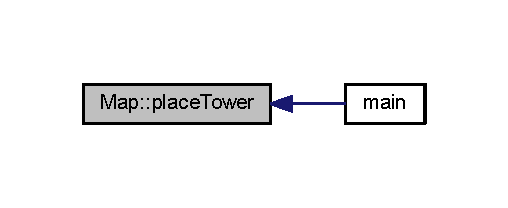
\includegraphics[width=244pt]{class_map_a0a7e6088ebbdc4fa9b82896841933014_icgraph}
\end{center}
\end{figure}




\subsection{Friends And Related Function Documentation}
\hypertarget{class_map_aebdb7e7ad7d1b28f8e1b3a0b0917bb9c}{\index{Map@{Map}!operator$<$$<$@{operator$<$$<$}}
\index{operator$<$$<$@{operator$<$$<$}!Map@{Map}}
\subsubsection[{operator$<$$<$}]{\setlength{\rightskip}{0pt plus 5cm}std\+::ostream\& operator$<$$<$ (
\begin{DoxyParamCaption}
\item[{std\+::ostream \&}]{output, }
\item[{const {\bf Map} \&}]{map}
\end{DoxyParamCaption}
)\hspace{0.3cm}{\ttfamily [friend]}}}\label{class_map_aebdb7e7ad7d1b28f8e1b3a0b0917bb9c}


Overloaded cout operator to print out Maps. 


\begin{DoxyParams}{Parameters}
{\em output} & Output stream address \\
\hline
{\em critter} & Const address to \hyperlink{class_map}{Map} \\
\hline
\end{DoxyParams}
\begin{DoxyReturn}{Returns}
Address to output stream 
\end{DoxyReturn}


\subsection{Member Data Documentation}
\hypertarget{class_map_aa5d63b554ad19c18cdc9911536e42001}{\index{Map@{Map}!map@{map}}
\index{map@{map}!Map@{Map}}
\subsubsection[{map}]{\setlength{\rightskip}{0pt plus 5cm}{\bf Map\+::\+Cell} Map\+::map\mbox{[}{\bf map\+\_\+size}\mbox{]}\mbox{[}{\bf map\+\_\+size}\mbox{]}}}\label{class_map_aa5d63b554ad19c18cdc9911536e42001}


2\+D array representing the map grid. 

\hypertarget{class_map_a6f922edb15340e98aee860d269e50703}{\index{Map@{Map}!map\+\_\+size@{map\+\_\+size}}
\index{map\+\_\+size@{map\+\_\+size}!Map@{Map}}
\subsubsection[{map\+\_\+size}]{\setlength{\rightskip}{0pt plus 5cm}const int Map\+::map\+\_\+size = 5\hspace{0.3cm}{\ttfamily [static]}}}\label{class_map_a6f922edb15340e98aee860d269e50703}


The documentation for this class was generated from the following file\+:\begin{DoxyCompactItemize}
\item 
C\+O\+M\+P345/\+Assignment1\+\_\+no\+G\+U\+I/\+Critter\+Group\+Generator/\+Critter\+Group\+Generator/include/\hyperlink{_map_8h}{Map.\+h}\end{DoxyCompactItemize}

\hypertarget{struct_map_1_1_path_cell}{\section{Map\+:\+:Path\+Cell Struct Reference}
\label{struct_map_1_1_path_cell}\index{Map\+::\+Path\+Cell@{Map\+::\+Path\+Cell}}
}


Derived from base struct \hyperlink{struct_map_1_1_cell}{Cell}.  




{\ttfamily \#include $<$Map.\+h$>$}



Inheritance diagram for Map\+:\+:Path\+Cell\+:
\nopagebreak
\begin{figure}[H]
\begin{center}
\leavevmode
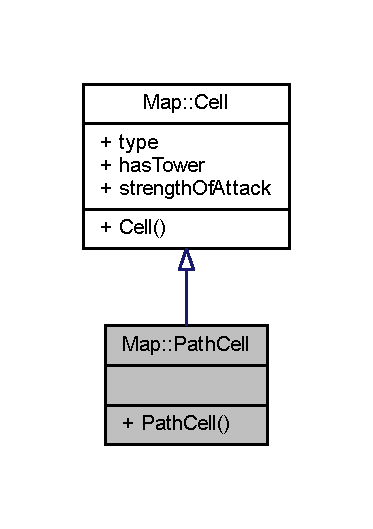
\includegraphics[width=179pt]{struct_map_1_1_path_cell__inherit__graph}
\end{center}
\end{figure}


Collaboration diagram for Map\+:\+:Path\+Cell\+:
\nopagebreak
\begin{figure}[H]
\begin{center}
\leavevmode
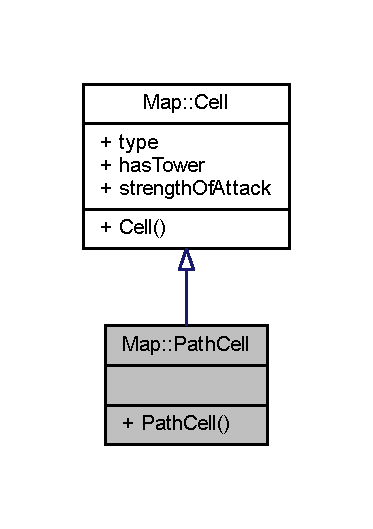
\includegraphics[width=179pt]{struct_map_1_1_path_cell__coll__graph}
\end{center}
\end{figure}
\subsection*{Public Member Functions}
\begin{DoxyCompactItemize}
\item 
\hyperlink{struct_map_1_1_path_cell_a4f7696c731d61dbd32da6b52fdb73381}{Path\+Cell} ()
\end{DoxyCompactItemize}
\subsection*{Additional Inherited Members}


\subsection{Detailed Description}
Derived from base struct \hyperlink{struct_map_1_1_cell}{Cell}. 

\subsection{Constructor \& Destructor Documentation}
\hypertarget{struct_map_1_1_path_cell_a4f7696c731d61dbd32da6b52fdb73381}{\index{Map\+::\+Path\+Cell@{Map\+::\+Path\+Cell}!Path\+Cell@{Path\+Cell}}
\index{Path\+Cell@{Path\+Cell}!Map\+::\+Path\+Cell@{Map\+::\+Path\+Cell}}
\subsubsection[{Path\+Cell}]{\setlength{\rightskip}{0pt plus 5cm}Map\+::\+Path\+Cell\+::\+Path\+Cell (
\begin{DoxyParamCaption}
{}
\end{DoxyParamCaption}
)\hspace{0.3cm}{\ttfamily [inline]}}}\label{struct_map_1_1_path_cell_a4f7696c731d61dbd32da6b52fdb73381}


The documentation for this struct was generated from the following file\+:\begin{DoxyCompactItemize}
\item 
C\+O\+M\+P345/\+Assignment1\+\_\+no\+G\+U\+I/\+Critter\+Group\+Generator/\+Critter\+Group\+Generator/include/\hyperlink{_map_8h}{Map.\+h}\end{DoxyCompactItemize}

\hypertarget{class_player}{\section{Player Class Reference}
\label{class_player}\index{Player@{Player}}
}


Class for \hyperlink{class_player}{Player}. Stub class of \hyperlink{class_player}{Player} for Critters.  




{\ttfamily \#include $<$Player.\+h$>$}



Collaboration diagram for Player\+:
\nopagebreak
\begin{figure}[H]
\begin{center}
\leavevmode
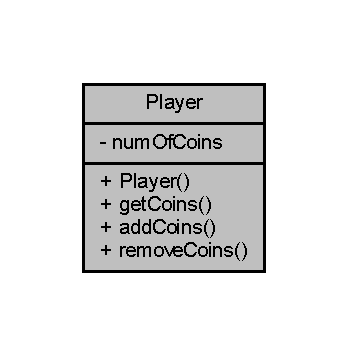
\includegraphics[width=167pt]{class_player__coll__graph}
\end{center}
\end{figure}
\subsection*{Public Member Functions}
\begin{DoxyCompactItemize}
\item 
\hyperlink{class_player_affe0cc3cb714f6deb4e62f0c0d3f1fd8}{Player} ()
\item 
int \hyperlink{class_player_a1b99d8f8f5f8230ae10cbed624c93e26}{get\+Coins} () const 
\item 
void \hyperlink{class_player_afb0f01357d0f7800e43bddeec32f3f41}{add\+Coins} (int coins)
\item 
void \hyperlink{class_player_a0a01dc7b78794fba8f38815f0e159a3a}{remove\+Coins} (int coins)
\end{DoxyCompactItemize}
\subsection*{Private Attributes}
\begin{DoxyCompactItemize}
\item 
int \hyperlink{class_player_ae76f51dc1a9a1356e41669cc4dcff55c}{num\+Of\+Coins}
\end{DoxyCompactItemize}
\subsection*{Friends}
\begin{DoxyCompactItemize}
\item 
std\+::ostream \& \hyperlink{class_player_af28e709121d213f58c0c593de95411c7}{operator$<$$<$} (std\+::ostream \&output, const \hyperlink{class_player}{Player} \&player)
\begin{DoxyCompactList}\small\item\em Overloaded cout operator to print out Playerss. \end{DoxyCompactList}\end{DoxyCompactItemize}


\subsection{Detailed Description}
Class for \hyperlink{class_player}{Player}. Stub class of \hyperlink{class_player}{Player} for Critters. 

\subsection{Constructor \& Destructor Documentation}
\hypertarget{class_player_affe0cc3cb714f6deb4e62f0c0d3f1fd8}{\index{Player@{Player}!Player@{Player}}
\index{Player@{Player}!Player@{Player}}
\subsubsection[{Player}]{\setlength{\rightskip}{0pt plus 5cm}Player\+::\+Player (
\begin{DoxyParamCaption}
{}
\end{DoxyParamCaption}
)\hspace{0.3cm}{\ttfamily [inline]}}}\label{class_player_affe0cc3cb714f6deb4e62f0c0d3f1fd8}


\subsection{Member Function Documentation}
\hypertarget{class_player_afb0f01357d0f7800e43bddeec32f3f41}{\index{Player@{Player}!add\+Coins@{add\+Coins}}
\index{add\+Coins@{add\+Coins}!Player@{Player}}
\subsubsection[{add\+Coins}]{\setlength{\rightskip}{0pt plus 5cm}void Player\+::add\+Coins (
\begin{DoxyParamCaption}
\item[{int}]{coins}
\end{DoxyParamCaption}
)\hspace{0.3cm}{\ttfamily [inline]}}}\label{class_player_afb0f01357d0f7800e43bddeec32f3f41}
\hypertarget{class_player_a1b99d8f8f5f8230ae10cbed624c93e26}{\index{Player@{Player}!get\+Coins@{get\+Coins}}
\index{get\+Coins@{get\+Coins}!Player@{Player}}
\subsubsection[{get\+Coins}]{\setlength{\rightskip}{0pt plus 5cm}int Player\+::get\+Coins (
\begin{DoxyParamCaption}
{}
\end{DoxyParamCaption}
) const\hspace{0.3cm}{\ttfamily [inline]}}}\label{class_player_a1b99d8f8f5f8230ae10cbed624c93e26}
\hypertarget{class_player_a0a01dc7b78794fba8f38815f0e159a3a}{\index{Player@{Player}!remove\+Coins@{remove\+Coins}}
\index{remove\+Coins@{remove\+Coins}!Player@{Player}}
\subsubsection[{remove\+Coins}]{\setlength{\rightskip}{0pt plus 5cm}void Player\+::remove\+Coins (
\begin{DoxyParamCaption}
\item[{int}]{coins}
\end{DoxyParamCaption}
)\hspace{0.3cm}{\ttfamily [inline]}}}\label{class_player_a0a01dc7b78794fba8f38815f0e159a3a}


Here is the caller graph for this function\+:
\nopagebreak
\begin{figure}[H]
\begin{center}
\leavevmode
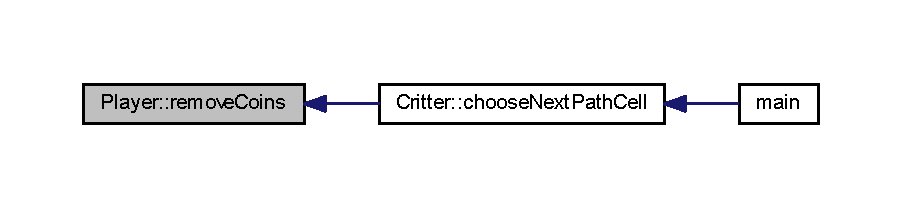
\includegraphics[width=350pt]{class_player_a0a01dc7b78794fba8f38815f0e159a3a_icgraph}
\end{center}
\end{figure}




\subsection{Friends And Related Function Documentation}
\hypertarget{class_player_af28e709121d213f58c0c593de95411c7}{\index{Player@{Player}!operator$<$$<$@{operator$<$$<$}}
\index{operator$<$$<$@{operator$<$$<$}!Player@{Player}}
\subsubsection[{operator$<$$<$}]{\setlength{\rightskip}{0pt plus 5cm}std\+::ostream\& operator$<$$<$ (
\begin{DoxyParamCaption}
\item[{std\+::ostream \&}]{output, }
\item[{const {\bf Player} \&}]{player}
\end{DoxyParamCaption}
)\hspace{0.3cm}{\ttfamily [friend]}}}\label{class_player_af28e709121d213f58c0c593de95411c7}


Overloaded cout operator to print out Playerss. 


\begin{DoxyParams}{Parameters}
{\em output} & Output stream address \\
\hline
{\em critter} & Const address to \hyperlink{class_player}{Player} \\
\hline
\end{DoxyParams}
\begin{DoxyReturn}{Returns}
Address to output stream 
\end{DoxyReturn}


\subsection{Member Data Documentation}
\hypertarget{class_player_ae76f51dc1a9a1356e41669cc4dcff55c}{\index{Player@{Player}!num\+Of\+Coins@{num\+Of\+Coins}}
\index{num\+Of\+Coins@{num\+Of\+Coins}!Player@{Player}}
\subsubsection[{num\+Of\+Coins}]{\setlength{\rightskip}{0pt plus 5cm}int Player\+::num\+Of\+Coins\hspace{0.3cm}{\ttfamily [private]}}}\label{class_player_ae76f51dc1a9a1356e41669cc4dcff55c}


The documentation for this class was generated from the following file\+:\begin{DoxyCompactItemize}
\item 
C\+O\+M\+P345/\+Assignment1\+\_\+no\+G\+U\+I/\+Critter\+Group\+Generator/\+Critter\+Group\+Generator/include/\hyperlink{_player_8h}{Player.\+h}\end{DoxyCompactItemize}

\hypertarget{struct_map_1_1_scenery_cell}{\section{Map\+:\+:Scenery\+Cell Struct Reference}
\label{struct_map_1_1_scenery_cell}\index{Map\+::\+Scenery\+Cell@{Map\+::\+Scenery\+Cell}}
}


Derived from base struct \hyperlink{struct_map_1_1_cell}{Cell}.  




{\ttfamily \#include $<$Map.\+h$>$}



Inheritance diagram for Map\+:\+:Scenery\+Cell\+:
\nopagebreak
\begin{figure}[H]
\begin{center}
\leavevmode
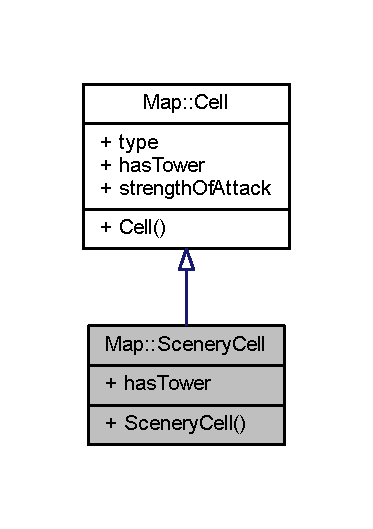
\includegraphics[width=179pt]{struct_map_1_1_scenery_cell__inherit__graph}
\end{center}
\end{figure}


Collaboration diagram for Map\+:\+:Scenery\+Cell\+:
\nopagebreak
\begin{figure}[H]
\begin{center}
\leavevmode
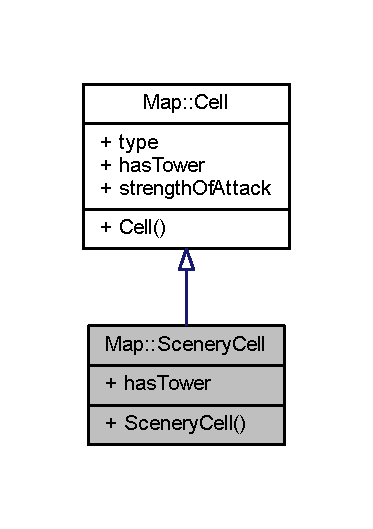
\includegraphics[width=179pt]{struct_map_1_1_scenery_cell__coll__graph}
\end{center}
\end{figure}
\subsection*{Public Member Functions}
\begin{DoxyCompactItemize}
\item 
\hyperlink{struct_map_1_1_scenery_cell_a117a6326d9265b3829e2110dfef8f04b}{Scenery\+Cell} ()
\end{DoxyCompactItemize}
\subsection*{Public Attributes}
\begin{DoxyCompactItemize}
\item 
bool \hyperlink{struct_map_1_1_scenery_cell_a29553a5fc8a9e9d228d91e66791c3d96}{has\+Tower}
\end{DoxyCompactItemize}


\subsection{Detailed Description}
Derived from base struct \hyperlink{struct_map_1_1_cell}{Cell}. 

\subsection{Constructor \& Destructor Documentation}
\hypertarget{struct_map_1_1_scenery_cell_a117a6326d9265b3829e2110dfef8f04b}{\index{Map\+::\+Scenery\+Cell@{Map\+::\+Scenery\+Cell}!Scenery\+Cell@{Scenery\+Cell}}
\index{Scenery\+Cell@{Scenery\+Cell}!Map\+::\+Scenery\+Cell@{Map\+::\+Scenery\+Cell}}
\subsubsection[{Scenery\+Cell}]{\setlength{\rightskip}{0pt plus 5cm}Map\+::\+Scenery\+Cell\+::\+Scenery\+Cell (
\begin{DoxyParamCaption}
{}
\end{DoxyParamCaption}
)\hspace{0.3cm}{\ttfamily [inline]}}}\label{struct_map_1_1_scenery_cell_a117a6326d9265b3829e2110dfef8f04b}


\subsection{Member Data Documentation}
\hypertarget{struct_map_1_1_scenery_cell_a29553a5fc8a9e9d228d91e66791c3d96}{\index{Map\+::\+Scenery\+Cell@{Map\+::\+Scenery\+Cell}!has\+Tower@{has\+Tower}}
\index{has\+Tower@{has\+Tower}!Map\+::\+Scenery\+Cell@{Map\+::\+Scenery\+Cell}}
\subsubsection[{has\+Tower}]{\setlength{\rightskip}{0pt plus 5cm}bool Map\+::\+Scenery\+Cell\+::has\+Tower}}\label{struct_map_1_1_scenery_cell_a29553a5fc8a9e9d228d91e66791c3d96}


The documentation for this struct was generated from the following file\+:\begin{DoxyCompactItemize}
\item 
C\+O\+M\+P345/\+Assignment1\+\_\+no\+G\+U\+I/\+Critter\+Group\+Generator/\+Critter\+Group\+Generator/include/\hyperlink{_map_8h}{Map.\+h}\end{DoxyCompactItemize}

\hypertarget{struct_map_1_1_start_cell}{\section{Map\+:\+:Start\+Cell Struct Reference}
\label{struct_map_1_1_start_cell}\index{Map\+::\+Start\+Cell@{Map\+::\+Start\+Cell}}
}


Derived from base struct \hyperlink{struct_map_1_1_cell}{Cell}.  




{\ttfamily \#include $<$Map.\+h$>$}



Inheritance diagram for Map\+:\+:Start\+Cell\+:
\nopagebreak
\begin{figure}[H]
\begin{center}
\leavevmode
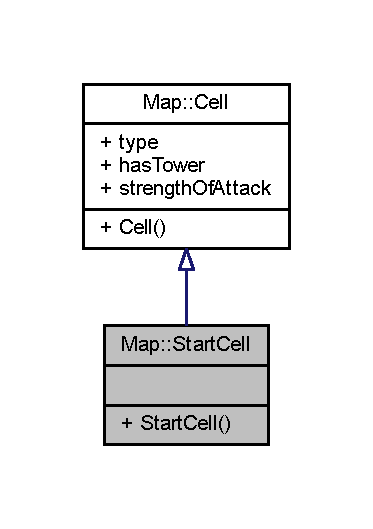
\includegraphics[width=179pt]{struct_map_1_1_start_cell__inherit__graph}
\end{center}
\end{figure}


Collaboration diagram for Map\+:\+:Start\+Cell\+:
\nopagebreak
\begin{figure}[H]
\begin{center}
\leavevmode
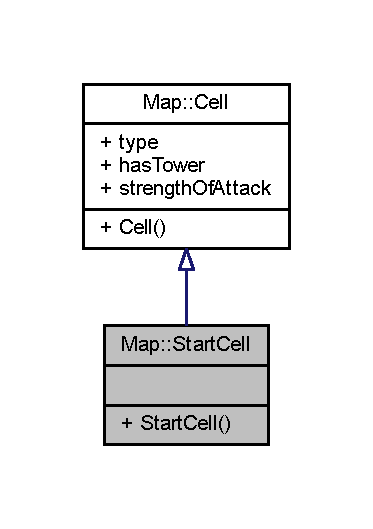
\includegraphics[width=179pt]{struct_map_1_1_start_cell__coll__graph}
\end{center}
\end{figure}
\subsection*{Public Member Functions}
\begin{DoxyCompactItemize}
\item 
\hyperlink{struct_map_1_1_start_cell_a7869384acd0dc391da806961f2885e30}{Start\+Cell} ()
\end{DoxyCompactItemize}
\subsection*{Additional Inherited Members}


\subsection{Detailed Description}
Derived from base struct \hyperlink{struct_map_1_1_cell}{Cell}. 

\subsection{Constructor \& Destructor Documentation}
\hypertarget{struct_map_1_1_start_cell_a7869384acd0dc391da806961f2885e30}{\index{Map\+::\+Start\+Cell@{Map\+::\+Start\+Cell}!Start\+Cell@{Start\+Cell}}
\index{Start\+Cell@{Start\+Cell}!Map\+::\+Start\+Cell@{Map\+::\+Start\+Cell}}
\subsubsection[{Start\+Cell}]{\setlength{\rightskip}{0pt plus 5cm}Map\+::\+Start\+Cell\+::\+Start\+Cell (
\begin{DoxyParamCaption}
{}
\end{DoxyParamCaption}
)\hspace{0.3cm}{\ttfamily [inline]}}}\label{struct_map_1_1_start_cell_a7869384acd0dc391da806961f2885e30}


The documentation for this struct was generated from the following file\+:\begin{DoxyCompactItemize}
\item 
C\+O\+M\+P345/\+Assignment1\+\_\+no\+G\+U\+I/\+Critter\+Group\+Generator/\+Critter\+Group\+Generator/include/\hyperlink{_map_8h}{Map.\+h}\end{DoxyCompactItemize}

\hypertarget{struct_map_1_1_tower_cell}{\section{Map\+:\+:Tower\+Cell Struct Reference}
\label{struct_map_1_1_tower_cell}\index{Map\+::\+Tower\+Cell@{Map\+::\+Tower\+Cell}}
}


Derived from base struct \hyperlink{struct_map_1_1_cell}{Cell}.  




{\ttfamily \#include $<$Map.\+h$>$}



Inheritance diagram for Map\+:\+:Tower\+Cell\+:
\nopagebreak
\begin{figure}[H]
\begin{center}
\leavevmode
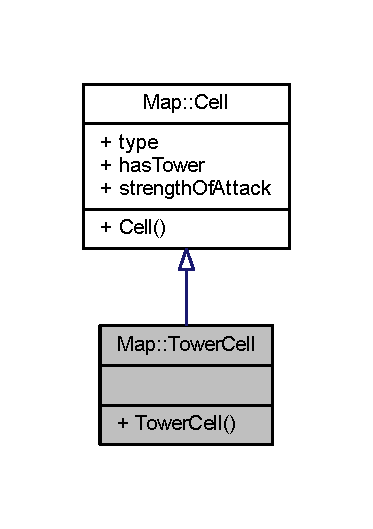
\includegraphics[width=179pt]{struct_map_1_1_tower_cell__inherit__graph}
\end{center}
\end{figure}


Collaboration diagram for Map\+:\+:Tower\+Cell\+:
\nopagebreak
\begin{figure}[H]
\begin{center}
\leavevmode
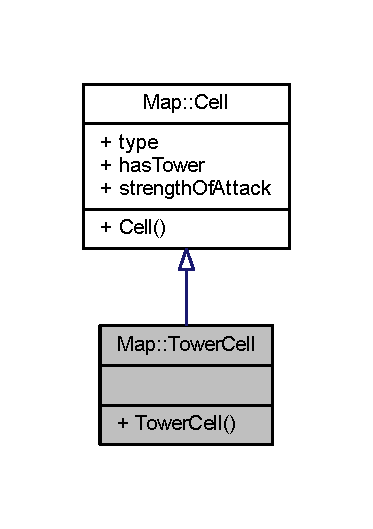
\includegraphics[width=179pt]{struct_map_1_1_tower_cell__coll__graph}
\end{center}
\end{figure}
\subsection*{Public Member Functions}
\begin{DoxyCompactItemize}
\item 
\hyperlink{struct_map_1_1_tower_cell_ae160f2d1ab399d634801e12b508ab5ef}{Tower\+Cell} ()
\end{DoxyCompactItemize}
\subsection*{Additional Inherited Members}


\subsection{Detailed Description}
Derived from base struct \hyperlink{struct_map_1_1_cell}{Cell}. 

\subsection{Constructor \& Destructor Documentation}
\hypertarget{struct_map_1_1_tower_cell_ae160f2d1ab399d634801e12b508ab5ef}{\index{Map\+::\+Tower\+Cell@{Map\+::\+Tower\+Cell}!Tower\+Cell@{Tower\+Cell}}
\index{Tower\+Cell@{Tower\+Cell}!Map\+::\+Tower\+Cell@{Map\+::\+Tower\+Cell}}
\subsubsection[{Tower\+Cell}]{\setlength{\rightskip}{0pt plus 5cm}Map\+::\+Tower\+Cell\+::\+Tower\+Cell (
\begin{DoxyParamCaption}
{}
\end{DoxyParamCaption}
)\hspace{0.3cm}{\ttfamily [inline]}}}\label{struct_map_1_1_tower_cell_ae160f2d1ab399d634801e12b508ab5ef}


The documentation for this struct was generated from the following file\+:\begin{DoxyCompactItemize}
\item 
C\+O\+M\+P345/\+Assignment1\+\_\+no\+G\+U\+I/\+Critter\+Group\+Generator/\+Critter\+Group\+Generator/include/\hyperlink{_map_8h}{Map.\+h}\end{DoxyCompactItemize}

\hypertarget{class_werecat}{\section{Werecat Class Reference}
\label{class_werecat}\index{Werecat@{Werecat}}
}


Class for \hyperlink{class_werecat}{Werecat}. Subclass of \hyperlink{class_critter}{Critter}.  




{\ttfamily \#include $<$Werecat.\+h$>$}



Inheritance diagram for Werecat\+:
\nopagebreak
\begin{figure}[H]
\begin{center}
\leavevmode
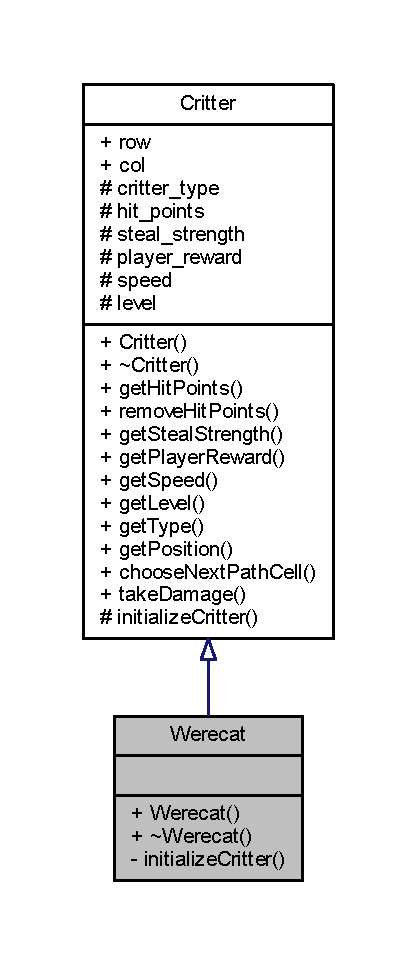
\includegraphics[width=200pt]{class_werecat__inherit__graph}
\end{center}
\end{figure}


Collaboration diagram for Werecat\+:
\nopagebreak
\begin{figure}[H]
\begin{center}
\leavevmode
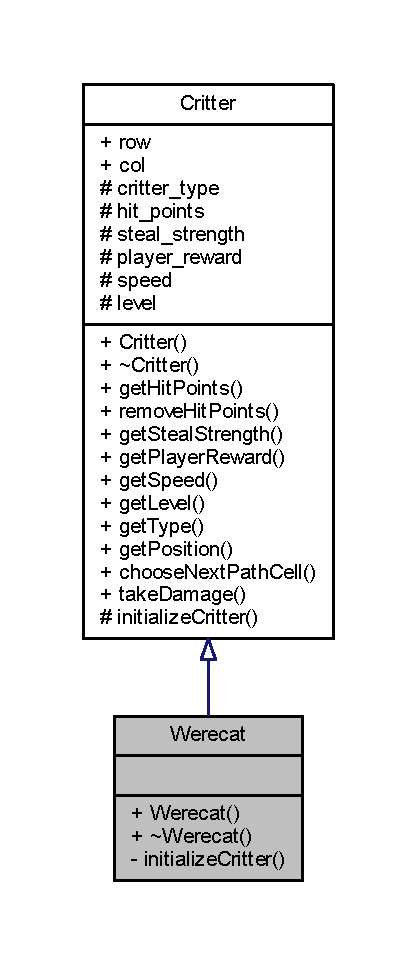
\includegraphics[width=200pt]{class_werecat__coll__graph}
\end{center}
\end{figure}
\subsection*{Public Member Functions}
\begin{DoxyCompactItemize}
\item 
\hyperlink{class_werecat_ab6533d29e63885a9599ed7c8605f998e}{Werecat} ()
\begin{DoxyCompactList}\small\item\em The \hyperlink{class_werecat}{Werecat} constructor. Calls \hyperlink{class_werecat_ae3c16d3ee0d96cb7ad7126cc3ae088a0}{initialize\+Critter()} to set attributes of the \hyperlink{class_werecat}{Werecat} object. \end{DoxyCompactList}\item 
\hyperlink{class_werecat_aa83431ddead97d0e43618c0fe6ac2551}{$\sim$\+Werecat} ()
\end{DoxyCompactItemize}
\subsection*{Private Member Functions}
\begin{DoxyCompactItemize}
\item 
virtual void \hyperlink{class_werecat_ae3c16d3ee0d96cb7ad7126cc3ae088a0}{initialize\+Critter} ()
\begin{DoxyCompactList}\small\item\em Initialization function for a \hyperlink{class_werecat}{Werecat}. \end{DoxyCompactList}\end{DoxyCompactItemize}
\subsection*{Additional Inherited Members}


\subsection{Detailed Description}
Class for \hyperlink{class_werecat}{Werecat}. Subclass of \hyperlink{class_critter}{Critter}. 

\subsection{Constructor \& Destructor Documentation}
\hypertarget{class_werecat_ab6533d29e63885a9599ed7c8605f998e}{\index{Werecat@{Werecat}!Werecat@{Werecat}}
\index{Werecat@{Werecat}!Werecat@{Werecat}}
\subsubsection[{Werecat}]{\setlength{\rightskip}{0pt plus 5cm}Werecat\+::\+Werecat (
\begin{DoxyParamCaption}
{}
\end{DoxyParamCaption}
)}}\label{class_werecat_ab6533d29e63885a9599ed7c8605f998e}


The \hyperlink{class_werecat}{Werecat} constructor. Calls \hyperlink{class_werecat_ae3c16d3ee0d96cb7ad7126cc3ae088a0}{initialize\+Critter()} to set attributes of the \hyperlink{class_werecat}{Werecat} object. 



Here is the call graph for this function\+:
\nopagebreak
\begin{figure}[H]
\begin{center}
\leavevmode
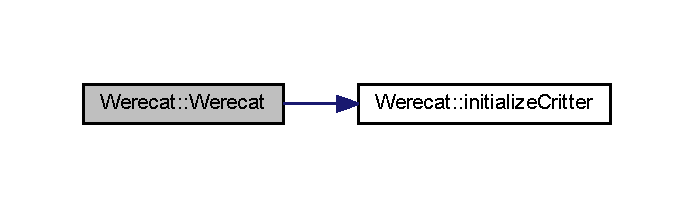
\includegraphics[width=333pt]{class_werecat_ab6533d29e63885a9599ed7c8605f998e_cgraph}
\end{center}
\end{figure}


\hypertarget{class_werecat_aa83431ddead97d0e43618c0fe6ac2551}{\index{Werecat@{Werecat}!````~Werecat@{$\sim$\+Werecat}}
\index{````~Werecat@{$\sim$\+Werecat}!Werecat@{Werecat}}
\subsubsection[{$\sim$\+Werecat}]{\setlength{\rightskip}{0pt plus 5cm}Werecat\+::$\sim$\+Werecat (
\begin{DoxyParamCaption}
{}
\end{DoxyParamCaption}
)\hspace{0.3cm}{\ttfamily [inline]}}}\label{class_werecat_aa83431ddead97d0e43618c0fe6ac2551}


\subsection{Member Function Documentation}
\hypertarget{class_werecat_ae3c16d3ee0d96cb7ad7126cc3ae088a0}{\index{Werecat@{Werecat}!initialize\+Critter@{initialize\+Critter}}
\index{initialize\+Critter@{initialize\+Critter}!Werecat@{Werecat}}
\subsubsection[{initialize\+Critter}]{\setlength{\rightskip}{0pt plus 5cm}void Werecat\+::initialize\+Critter (
\begin{DoxyParamCaption}
{}
\end{DoxyParamCaption}
)\hspace{0.3cm}{\ttfamily [private]}, {\ttfamily [virtual]}}}\label{class_werecat_ae3c16d3ee0d96cb7ad7126cc3ae088a0}


Initialization function for a \hyperlink{class_werecat}{Werecat}. 

\begin{DoxyReturn}{Returns}
Void.
\end{DoxyReturn}
Initialization specific to a \hyperlink{class_werecat}{Werecat} object 

Implements \hyperlink{class_critter_ab903f6d28ef3fc70808390fef8816b79}{Critter}.



Here is the caller graph for this function\+:
\nopagebreak
\begin{figure}[H]
\begin{center}
\leavevmode
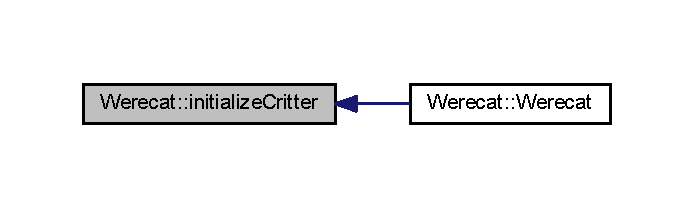
\includegraphics[width=333pt]{class_werecat_ae3c16d3ee0d96cb7ad7126cc3ae088a0_icgraph}
\end{center}
\end{figure}




The documentation for this class was generated from the following files\+:\begin{DoxyCompactItemize}
\item 
C\+O\+M\+P345/\+Assignment1\+\_\+no\+G\+U\+I/\+Critter\+Group\+Generator/\+Critter\+Group\+Generator/include/\hyperlink{_werecat_8h}{Werecat.\+h}\item 
C\+O\+M\+P345/\+Assignment1\+\_\+no\+G\+U\+I/\+Critter\+Group\+Generator/\+Critter\+Group\+Generator/src/game\+Objects/\hyperlink{_werecat_8cpp}{Werecat.\+cpp}\end{DoxyCompactItemize}

\hypertarget{class_werewolf}{\section{Werewolf Class Reference}
\label{class_werewolf}\index{Werewolf@{Werewolf}}
}


Class for \hyperlink{class_werewolf}{Werewolf}. Subclass of \hyperlink{class_critter}{Critter}.  




{\ttfamily \#include $<$Werewolf.\+h$>$}



Inheritance diagram for Werewolf\+:
\nopagebreak
\begin{figure}[H]
\begin{center}
\leavevmode
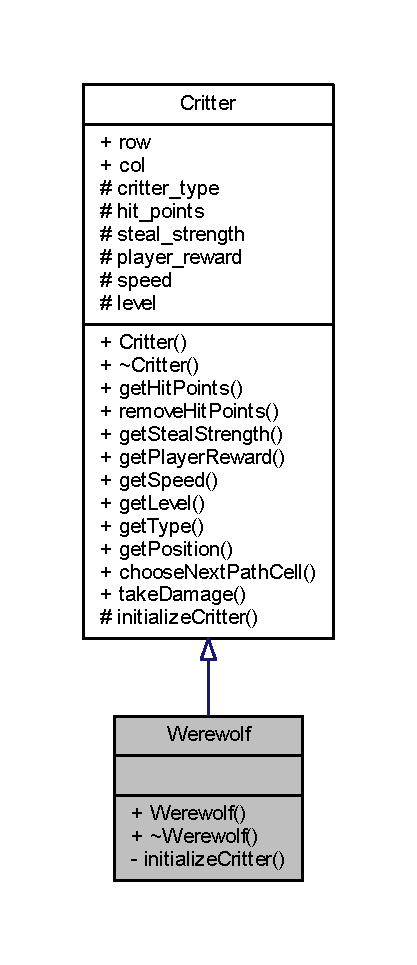
\includegraphics[width=200pt]{class_werewolf__inherit__graph}
\end{center}
\end{figure}


Collaboration diagram for Werewolf\+:
\nopagebreak
\begin{figure}[H]
\begin{center}
\leavevmode
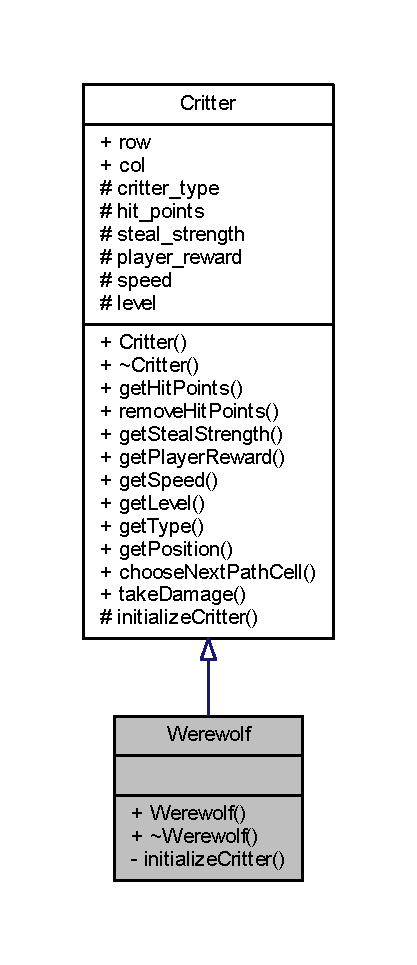
\includegraphics[width=200pt]{class_werewolf__coll__graph}
\end{center}
\end{figure}
\subsection*{Public Member Functions}
\begin{DoxyCompactItemize}
\item 
\hyperlink{class_werewolf_a56f3c77343deae2f8c4e9c39eeaf9ef4}{Werewolf} ()
\begin{DoxyCompactList}\small\item\em The \hyperlink{class_werecat}{Werecat} constructor. Calls \hyperlink{class_werewolf_afc8553cf4e3e33a609ca08c084d66ce0}{initialize\+Critter()} to set attributes of the \hyperlink{class_werecat}{Werecat} object. \end{DoxyCompactList}\item 
\hyperlink{class_werewolf_afa77a1212c2df2e1302ac6d769c67076}{$\sim$\+Werewolf} ()
\end{DoxyCompactItemize}
\subsection*{Private Member Functions}
\begin{DoxyCompactItemize}
\item 
virtual void \hyperlink{class_werewolf_afc8553cf4e3e33a609ca08c084d66ce0}{initialize\+Critter} ()
\begin{DoxyCompactList}\small\item\em Initialization function for a \hyperlink{class_werewolf}{Werewolf}. \end{DoxyCompactList}\end{DoxyCompactItemize}
\subsection*{Additional Inherited Members}


\subsection{Detailed Description}
Class for \hyperlink{class_werewolf}{Werewolf}. Subclass of \hyperlink{class_critter}{Critter}. 

\subsection{Constructor \& Destructor Documentation}
\hypertarget{class_werewolf_a56f3c77343deae2f8c4e9c39eeaf9ef4}{\index{Werewolf@{Werewolf}!Werewolf@{Werewolf}}
\index{Werewolf@{Werewolf}!Werewolf@{Werewolf}}
\subsubsection[{Werewolf}]{\setlength{\rightskip}{0pt plus 5cm}Werewolf\+::\+Werewolf (
\begin{DoxyParamCaption}
{}
\end{DoxyParamCaption}
)}}\label{class_werewolf_a56f3c77343deae2f8c4e9c39eeaf9ef4}


The \hyperlink{class_werecat}{Werecat} constructor. Calls \hyperlink{class_werewolf_afc8553cf4e3e33a609ca08c084d66ce0}{initialize\+Critter()} to set attributes of the \hyperlink{class_werecat}{Werecat} object. 



Here is the call graph for this function\+:
\nopagebreak
\begin{figure}[H]
\begin{center}
\leavevmode
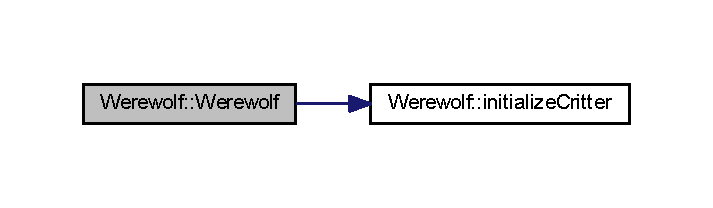
\includegraphics[width=342pt]{class_werewolf_a56f3c77343deae2f8c4e9c39eeaf9ef4_cgraph}
\end{center}
\end{figure}


\hypertarget{class_werewolf_afa77a1212c2df2e1302ac6d769c67076}{\index{Werewolf@{Werewolf}!````~Werewolf@{$\sim$\+Werewolf}}
\index{````~Werewolf@{$\sim$\+Werewolf}!Werewolf@{Werewolf}}
\subsubsection[{$\sim$\+Werewolf}]{\setlength{\rightskip}{0pt plus 5cm}Werewolf\+::$\sim$\+Werewolf (
\begin{DoxyParamCaption}
{}
\end{DoxyParamCaption}
)\hspace{0.3cm}{\ttfamily [inline]}}}\label{class_werewolf_afa77a1212c2df2e1302ac6d769c67076}


\subsection{Member Function Documentation}
\hypertarget{class_werewolf_afc8553cf4e3e33a609ca08c084d66ce0}{\index{Werewolf@{Werewolf}!initialize\+Critter@{initialize\+Critter}}
\index{initialize\+Critter@{initialize\+Critter}!Werewolf@{Werewolf}}
\subsubsection[{initialize\+Critter}]{\setlength{\rightskip}{0pt plus 5cm}void Werewolf\+::initialize\+Critter (
\begin{DoxyParamCaption}
{}
\end{DoxyParamCaption}
)\hspace{0.3cm}{\ttfamily [private]}, {\ttfamily [virtual]}}}\label{class_werewolf_afc8553cf4e3e33a609ca08c084d66ce0}


Initialization function for a \hyperlink{class_werewolf}{Werewolf}. 

\begin{DoxyReturn}{Returns}
Void.
\end{DoxyReturn}
Initialization specific to a \hyperlink{class_werewolf}{Werewolf} object 

Implements \hyperlink{class_critter_ab903f6d28ef3fc70808390fef8816b79}{Critter}.



Here is the caller graph for this function\+:
\nopagebreak
\begin{figure}[H]
\begin{center}
\leavevmode
\includegraphics[width=342pt]{class_werewolf_afc8553cf4e3e33a609ca08c084d66ce0_icgraph}
\end{center}
\end{figure}




The documentation for this class was generated from the following files\+:\begin{DoxyCompactItemize}
\item 
C\+O\+M\+P345/\+Assignment1\+\_\+no\+G\+U\+I/\+Critter\+Group\+Generator/\+Critter\+Group\+Generator/include/\hyperlink{_werewolf_8h}{Werewolf.\+h}\item 
C\+O\+M\+P345/\+Assignment1\+\_\+no\+G\+U\+I/\+Critter\+Group\+Generator/\+Critter\+Group\+Generator/src/game\+Objects/\hyperlink{_werewolf_8cpp}{Werewolf.\+cpp}\end{DoxyCompactItemize}

\chapter{File Documentation}
\hypertarget{_cat_8h}{\section{C\+O\+M\+P345/\+Assignment1\+\_\+no\+G\+U\+I/\+Critter\+Group\+Generator/\+Critter\+Group\+Generator/include/\+Cat.h File Reference}
\label{_cat_8h}\index{C\+O\+M\+P345/\+Assignment1\+\_\+no\+G\+U\+I/\+Critter\+Group\+Generator/\+Critter\+Group\+Generator/include/\+Cat.\+h@{C\+O\+M\+P345/\+Assignment1\+\_\+no\+G\+U\+I/\+Critter\+Group\+Generator/\+Critter\+Group\+Generator/include/\+Cat.\+h}}
}


Representation of \hyperlink{class_cat}{Cat} object.  


{\ttfamily \#include $<$Critter.\+h$>$}\\*
Include dependency graph for Cat.\+h\+:
\nopagebreak
\begin{figure}[H]
\begin{center}
\leavevmode
\includegraphics[width=255pt]{_cat_8h__incl}
\end{center}
\end{figure}
This graph shows which files directly or indirectly include this file\+:
\nopagebreak
\begin{figure}[H]
\begin{center}
\leavevmode
\includegraphics[width=350pt]{_cat_8h__dep__incl}
\end{center}
\end{figure}
\subsection*{Classes}
\begin{DoxyCompactItemize}
\item 
class \hyperlink{class_cat}{Cat}
\begin{DoxyCompactList}\small\item\em Class for \hyperlink{class_cat}{Cat}. Subclass of \hyperlink{class_critter}{Critter}. \end{DoxyCompactList}\end{DoxyCompactItemize}


\subsection{Detailed Description}
Representation of \hyperlink{class_cat}{Cat} object. 

This is the representation of the \hyperlink{class_cat}{Cat} object.

\begin{DoxyAuthor}{Author}
Stephanie Li 
\end{DoxyAuthor}

\hypertarget{_critter_8h}{\section{C\+O\+M\+P345/\+Assignment1\+\_\+no\+G\+U\+I/\+Critter\+Group\+Generator/\+Critter\+Group\+Generator/include/\+Critter.h File Reference}
\label{_critter_8h}\index{C\+O\+M\+P345/\+Assignment1\+\_\+no\+G\+U\+I/\+Critter\+Group\+Generator/\+Critter\+Group\+Generator/include/\+Critter.\+h@{C\+O\+M\+P345/\+Assignment1\+\_\+no\+G\+U\+I/\+Critter\+Group\+Generator/\+Critter\+Group\+Generator/include/\+Critter.\+h}}
}


Representation of critter object.  


{\ttfamily \#include $<$iostream$>$}\\*
{\ttfamily \#include $<$string$>$}\\*
{\ttfamily \#include $<$Map.\+h$>$}\\*
{\ttfamily \#include $<$Player.\+h$>$}\\*
Include dependency graph for Critter.\+h\+:
\nopagebreak
\begin{figure}[H]
\begin{center}
\leavevmode
\includegraphics[width=229pt]{_critter_8h__incl}
\end{center}
\end{figure}
This graph shows which files directly or indirectly include this file\+:
\nopagebreak
\begin{figure}[H]
\begin{center}
\leavevmode
\includegraphics[width=350pt]{_critter_8h__dep__incl}
\end{center}
\end{figure}
\subsection*{Classes}
\begin{DoxyCompactItemize}
\item 
class \hyperlink{class_critter}{Critter}
\begin{DoxyCompactList}\small\item\em Abstract base class of all Critters \hyperlink{class_critter}{Critter} defines the attributes, accessors, and update function for its subclass instances. \end{DoxyCompactList}\end{DoxyCompactItemize}


\subsection{Detailed Description}
Representation of critter object. 

This is the abstract representation of the critter object.

\begin{DoxyAuthor}{Author}
Stephanie Li 
\end{DoxyAuthor}

\hypertarget{_critter_factory_8h}{\section{C\+O\+M\+P345/\+Assignment1\+\_\+no\+G\+U\+I/\+Critter\+Group\+Generator/\+Critter\+Group\+Generator/include/\+Critter\+Factory.h File Reference}
\label{_critter_factory_8h}\index{C\+O\+M\+P345/\+Assignment1\+\_\+no\+G\+U\+I/\+Critter\+Group\+Generator/\+Critter\+Group\+Generator/include/\+Critter\+Factory.\+h@{C\+O\+M\+P345/\+Assignment1\+\_\+no\+G\+U\+I/\+Critter\+Group\+Generator/\+Critter\+Group\+Generator/include/\+Critter\+Factory.\+h}}
}


File for \hyperlink{class_critter_factory}{Critter\+Factory} class.  


{\ttfamily \#include $<$Critter.\+h$>$}\\*
{\ttfamily \#include $<$Cat.\+h$>$}\\*
{\ttfamily \#include $<$Dog.\+h$>$}\\*
{\ttfamily \#include $<$Werecat.\+h$>$}\\*
{\ttfamily \#include $<$Werewolf.\+h$>$}\\*
Include dependency graph for Critter\+Factory.\+h\+:
\nopagebreak
\begin{figure}[H]
\begin{center}
\leavevmode
\includegraphics[width=350pt]{_critter_factory_8h__incl}
\end{center}
\end{figure}
This graph shows which files directly or indirectly include this file\+:
\nopagebreak
\begin{figure}[H]
\begin{center}
\leavevmode
\includegraphics[width=350pt]{_critter_factory_8h__dep__incl}
\end{center}
\end{figure}
\subsection*{Classes}
\begin{DoxyCompactItemize}
\item 
class \hyperlink{class_critter_factory}{Critter\+Factory}
\begin{DoxyCompactList}\small\item\em Creates objects derived from \hyperlink{class_critter}{Critter}. Utility class that creates instance of a \hyperlink{class_critter}{Critter} subclass from a family of derived \hyperlink{class_critter}{Critter} classes. \end{DoxyCompactList}\end{DoxyCompactItemize}


\subsection{Detailed Description}
File for \hyperlink{class_critter_factory}{Critter\+Factory} class. 

\begin{DoxyAuthor}{Author}
Stephanie Li 
\end{DoxyAuthor}

\hypertarget{_critter_wave_8h}{\section{C\+O\+M\+P345/\+Assignment1\+\_\+no\+G\+U\+I/\+Critter\+Group\+Generator/\+Critter\+Group\+Generator/include/\+Critter\+Wave.h File Reference}
\label{_critter_wave_8h}\index{C\+O\+M\+P345/\+Assignment1\+\_\+no\+G\+U\+I/\+Critter\+Group\+Generator/\+Critter\+Group\+Generator/include/\+Critter\+Wave.\+h@{C\+O\+M\+P345/\+Assignment1\+\_\+no\+G\+U\+I/\+Critter\+Group\+Generator/\+Critter\+Group\+Generator/include/\+Critter\+Wave.\+h}}
}


File for \hyperlink{class_critter_wave}{Critter\+Wave} class.  


{\ttfamily \#include $<$Critter.\+h$>$}\\*
{\ttfamily \#include $<$Critter\+Factory.\+h$>$}\\*
{\ttfamily \#include $<$map$>$}\\*
{\ttfamily \#include $<$algorithm$>$}\\*
Include dependency graph for Critter\+Wave.\+h\+:
\nopagebreak
\begin{figure}[H]
\begin{center}
\leavevmode
\includegraphics[width=350pt]{_critter_wave_8h__incl}
\end{center}
\end{figure}
This graph shows which files directly or indirectly include this file\+:
\nopagebreak
\begin{figure}[H]
\begin{center}
\leavevmode
\includegraphics[width=350pt]{_critter_wave_8h__dep__incl}
\end{center}
\end{figure}
\subsection*{Classes}
\begin{DoxyCompactItemize}
\item 
class \hyperlink{class_critter_wave}{Critter\+Wave}
\begin{DoxyCompactList}\small\item\em Represents a wave of Critters. Class that has holds Critters in a map data structure, which represents a wave of Critters. \end{DoxyCompactList}\item 
struct \hyperlink{struct_critter_wave_1_1_critter_wave_deallocator}{Critter\+Wave\+::\+Critter\+Wave\+Deallocator}
\begin{DoxyCompactList}\small\item\em Struct deallocating resources used in a \hyperlink{class_critter_wave}{Critter\+Wave} map. \end{DoxyCompactList}\end{DoxyCompactItemize}


\subsection{Detailed Description}
File for \hyperlink{class_critter_wave}{Critter\+Wave} class. 

\begin{DoxyAuthor}{Author}
Stephanie Li 
\end{DoxyAuthor}

\hypertarget{_dog_8h}{\section{C\+O\+M\+P345/\+Assignment1\+\_\+no\+G\+U\+I/\+Critter\+Group\+Generator/\+Critter\+Group\+Generator/include/\+Dog.h File Reference}
\label{_dog_8h}\index{C\+O\+M\+P345/\+Assignment1\+\_\+no\+G\+U\+I/\+Critter\+Group\+Generator/\+Critter\+Group\+Generator/include/\+Dog.\+h@{C\+O\+M\+P345/\+Assignment1\+\_\+no\+G\+U\+I/\+Critter\+Group\+Generator/\+Critter\+Group\+Generator/include/\+Dog.\+h}}
}


Representation of \hyperlink{class_dog}{Dog} object.  


{\ttfamily \#include $<$Critter.\+h$>$}\\*
Include dependency graph for Dog.\+h\+:
\nopagebreak
\begin{figure}[H]
\begin{center}
\leavevmode
\includegraphics[width=257pt]{_dog_8h__incl}
\end{center}
\end{figure}
This graph shows which files directly or indirectly include this file\+:
\nopagebreak
\begin{figure}[H]
\begin{center}
\leavevmode
\includegraphics[width=350pt]{_dog_8h__dep__incl}
\end{center}
\end{figure}
\subsection*{Classes}
\begin{DoxyCompactItemize}
\item 
class \hyperlink{class_dog}{Dog}
\begin{DoxyCompactList}\small\item\em Class for \hyperlink{class_dog}{Dog}. Subclass of \hyperlink{class_critter}{Critter}. \end{DoxyCompactList}\end{DoxyCompactItemize}


\subsection{Detailed Description}
Representation of \hyperlink{class_dog}{Dog} object. 

This is the representation of the \hyperlink{class_dog}{Dog} object.

\begin{DoxyAuthor}{Author}
Stephanie Li 
\end{DoxyAuthor}

\hypertarget{_map_8h}{\section{C\+O\+M\+P345/\+Assignment1\+\_\+no\+G\+U\+I/\+Critter\+Group\+Generator/\+Critter\+Group\+Generator/include/\+Map.h File Reference}
\label{_map_8h}\index{C\+O\+M\+P345/\+Assignment1\+\_\+no\+G\+U\+I/\+Critter\+Group\+Generator/\+Critter\+Group\+Generator/include/\+Map.\+h@{C\+O\+M\+P345/\+Assignment1\+\_\+no\+G\+U\+I/\+Critter\+Group\+Generator/\+Critter\+Group\+Generator/include/\+Map.\+h}}
}


Representation of \hyperlink{class_map}{Map} object.  


{\ttfamily \#include $<$iostream$>$}\\*
{\ttfamily \#include $<$string$>$}\\*
Include dependency graph for Map.\+h\+:
\nopagebreak
\begin{figure}[H]
\begin{center}
\leavevmode
\includegraphics[width=259pt]{_map_8h__incl}
\end{center}
\end{figure}
This graph shows which files directly or indirectly include this file\+:
\nopagebreak
\begin{figure}[H]
\begin{center}
\leavevmode
\includegraphics[width=350pt]{_map_8h__dep__incl}
\end{center}
\end{figure}
\subsection*{Classes}
\begin{DoxyCompactItemize}
\item 
class \hyperlink{class_map}{Map}
\begin{DoxyCompactList}\small\item\em Class for \hyperlink{class_map}{Map}. Stub class of map for Critters. \end{DoxyCompactList}\item 
struct \hyperlink{struct_map_1_1_cell}{Map\+::\+Cell}
\begin{DoxyCompactList}\small\item\em Base struct for \hyperlink{struct_map_1_1_cell}{Cell} objects in a \hyperlink{class_map}{Map}. \end{DoxyCompactList}\item 
struct \hyperlink{struct_map_1_1_scenery_cell}{Map\+::\+Scenery\+Cell}
\begin{DoxyCompactList}\small\item\em Derived from base struct \hyperlink{struct_map_1_1_cell}{Cell}. \end{DoxyCompactList}\item 
struct \hyperlink{struct_map_1_1_path_cell}{Map\+::\+Path\+Cell}
\begin{DoxyCompactList}\small\item\em Derived from base struct \hyperlink{struct_map_1_1_cell}{Cell}. \end{DoxyCompactList}\item 
struct \hyperlink{struct_map_1_1_start_cell}{Map\+::\+Start\+Cell}
\begin{DoxyCompactList}\small\item\em Derived from base struct \hyperlink{struct_map_1_1_cell}{Cell}. \end{DoxyCompactList}\item 
struct \hyperlink{struct_map_1_1_exit_cell}{Map\+::\+Exit\+Cell}
\begin{DoxyCompactList}\small\item\em Derived from base struct \hyperlink{struct_map_1_1_cell}{Cell}. \end{DoxyCompactList}\item 
struct \hyperlink{struct_map_1_1_tower_cell}{Map\+::\+Tower\+Cell}
\begin{DoxyCompactList}\small\item\em Derived from base struct \hyperlink{struct_map_1_1_cell}{Cell}. \end{DoxyCompactList}\end{DoxyCompactItemize}


\subsection{Detailed Description}
Representation of \hyperlink{class_map}{Map} object. 

This is the representation of the \hyperlink{class_map}{Map} object.

\begin{DoxyAuthor}{Author}
Stephanie Li 
\end{DoxyAuthor}

\hypertarget{_player_8h}{\section{C\+O\+M\+P345/\+Assignment1\+\_\+no\+G\+U\+I/\+Critter\+Group\+Generator/\+Critter\+Group\+Generator/include/\+Player.h File Reference}
\label{_player_8h}\index{C\+O\+M\+P345/\+Assignment1\+\_\+no\+G\+U\+I/\+Critter\+Group\+Generator/\+Critter\+Group\+Generator/include/\+Player.\+h@{C\+O\+M\+P345/\+Assignment1\+\_\+no\+G\+U\+I/\+Critter\+Group\+Generator/\+Critter\+Group\+Generator/include/\+Player.\+h}}
}


Representation of \hyperlink{class_player}{Player} object.  


{\ttfamily \#include $<$iostream$>$}\\*
{\ttfamily \#include $<$string$>$}\\*
Include dependency graph for Player.\+h\+:
\nopagebreak
\begin{figure}[H]
\begin{center}
\leavevmode
\includegraphics[width=229pt]{_player_8h__incl}
\end{center}
\end{figure}
This graph shows which files directly or indirectly include this file\+:
\nopagebreak
\begin{figure}[H]
\begin{center}
\leavevmode
\includegraphics[width=350pt]{_player_8h__dep__incl}
\end{center}
\end{figure}
\subsection*{Classes}
\begin{DoxyCompactItemize}
\item 
class \hyperlink{class_player}{Player}
\begin{DoxyCompactList}\small\item\em Class for \hyperlink{class_player}{Player}. Stub class of \hyperlink{class_player}{Player} for Critters. \end{DoxyCompactList}\end{DoxyCompactItemize}


\subsection{Detailed Description}
Representation of \hyperlink{class_player}{Player} object. 

This is the representation of the \hyperlink{class_player}{Player} object.

\begin{DoxyAuthor}{Author}
Stephanie Li 
\end{DoxyAuthor}

\hypertarget{_werecat_8h}{\section{C\+O\+M\+P345/\+Assignment1\+\_\+no\+G\+U\+I/\+Critter\+Group\+Generator/\+Critter\+Group\+Generator/include/\+Werecat.h File Reference}
\label{_werecat_8h}\index{C\+O\+M\+P345/\+Assignment1\+\_\+no\+G\+U\+I/\+Critter\+Group\+Generator/\+Critter\+Group\+Generator/include/\+Werecat.\+h@{C\+O\+M\+P345/\+Assignment1\+\_\+no\+G\+U\+I/\+Critter\+Group\+Generator/\+Critter\+Group\+Generator/include/\+Werecat.\+h}}
}


Representation of \hyperlink{class_werecat}{Werecat} object.  


{\ttfamily \#include $<$Critter.\+h$>$}\\*
Include dependency graph for Werecat.\+h\+:
\nopagebreak
\begin{figure}[H]
\begin{center}
\leavevmode
\includegraphics[width=229pt]{_werecat_8h__incl}
\end{center}
\end{figure}
This graph shows which files directly or indirectly include this file\+:
\nopagebreak
\begin{figure}[H]
\begin{center}
\leavevmode
\includegraphics[width=350pt]{_werecat_8h__dep__incl}
\end{center}
\end{figure}
\subsection*{Classes}
\begin{DoxyCompactItemize}
\item 
class \hyperlink{class_werecat}{Werecat}
\begin{DoxyCompactList}\small\item\em Class for \hyperlink{class_werecat}{Werecat}. Subclass of \hyperlink{class_critter}{Critter}. \end{DoxyCompactList}\end{DoxyCompactItemize}


\subsection{Detailed Description}
Representation of \hyperlink{class_werecat}{Werecat} object. 

This is the representation of the \hyperlink{class_werecat}{Werecat} object.

\begin{DoxyAuthor}{Author}
Stephanie Li 
\end{DoxyAuthor}

\hypertarget{_werewolf_8h}{\section{C\+O\+M\+P345/\+Assignment1\+\_\+no\+G\+U\+I/\+Critter\+Group\+Generator/\+Critter\+Group\+Generator/include/\+Werewolf.h File Reference}
\label{_werewolf_8h}\index{C\+O\+M\+P345/\+Assignment1\+\_\+no\+G\+U\+I/\+Critter\+Group\+Generator/\+Critter\+Group\+Generator/include/\+Werewolf.\+h@{C\+O\+M\+P345/\+Assignment1\+\_\+no\+G\+U\+I/\+Critter\+Group\+Generator/\+Critter\+Group\+Generator/include/\+Werewolf.\+h}}
}


Representation of \hyperlink{class_werewolf}{Werewolf} object.  


{\ttfamily \#include $<$Critter.\+h$>$}\\*
Include dependency graph for Werewolf.\+h\+:
\nopagebreak
\begin{figure}[H]
\begin{center}
\leavevmode
\includegraphics[width=229pt]{_werewolf_8h__incl}
\end{center}
\end{figure}
This graph shows which files directly or indirectly include this file\+:
\nopagebreak
\begin{figure}[H]
\begin{center}
\leavevmode
\includegraphics[width=350pt]{_werewolf_8h__dep__incl}
\end{center}
\end{figure}
\subsection*{Classes}
\begin{DoxyCompactItemize}
\item 
class \hyperlink{class_werewolf}{Werewolf}
\begin{DoxyCompactList}\small\item\em Class for \hyperlink{class_werewolf}{Werewolf}. Subclass of \hyperlink{class_critter}{Critter}. \end{DoxyCompactList}\end{DoxyCompactItemize}


\subsection{Detailed Description}
Representation of \hyperlink{class_werewolf}{Werewolf} object. 

This is the representation of the \hyperlink{class_werewolf}{Werewolf} object.

\begin{DoxyAuthor}{Author}
Stephanie Li 
\end{DoxyAuthor}

\hypertarget{_driver_8cpp}{\section{C\+O\+M\+P345/\+Assignment1\+\_\+no\+G\+U\+I/\+Critter\+Group\+Generator/\+Critter\+Group\+Generator/src/\+Driver.cpp File Reference}
\label{_driver_8cpp}\index{C\+O\+M\+P345/\+Assignment1\+\_\+no\+G\+U\+I/\+Critter\+Group\+Generator/\+Critter\+Group\+Generator/src/\+Driver.\+cpp@{C\+O\+M\+P345/\+Assignment1\+\_\+no\+G\+U\+I/\+Critter\+Group\+Generator/\+Critter\+Group\+Generator/src/\+Driver.\+cpp}}
}
{\ttfamily \#include $<$iostream$>$}\\*
{\ttfamily \#include $<$string$>$}\\*
{\ttfamily \#include $<$Critter\+Factory.\+h$>$}\\*
{\ttfamily \#include $<$Critter\+Wave.\+h$>$}\\*
{\ttfamily \#include $<$Map.\+h$>$}\\*
{\ttfamily \#include $<$Player.\+h$>$}\\*
Include dependency graph for Driver.\+cpp\+:
\nopagebreak
\begin{figure}[H]
\begin{center}
\leavevmode
\includegraphics[width=350pt]{_driver_8cpp__incl}
\end{center}
\end{figure}
\subsection*{Functions}
\begin{DoxyCompactItemize}
\item 
int \hyperlink{_driver_8cpp_a17c71e8de8c58645dd41431d716ac739}{main} (int argc, char $\ast$$\ast$argv\mbox{[}$\,$\mbox{]})
\end{DoxyCompactItemize}


\subsection{Function Documentation}
\hypertarget{_driver_8cpp_a17c71e8de8c58645dd41431d716ac739}{\index{Driver.\+cpp@{Driver.\+cpp}!main@{main}}
\index{main@{main}!Driver.\+cpp@{Driver.\+cpp}}
\subsubsection[{main}]{\setlength{\rightskip}{0pt plus 5cm}int main (
\begin{DoxyParamCaption}
\item[{int}]{argc, }
\item[{char $\ast$$\ast$}]{argv\mbox{[}$\,$\mbox{]}}
\end{DoxyParamCaption}
)}}\label{_driver_8cpp_a17c71e8de8c58645dd41431d716ac739}


Here is the call graph for this function\+:
\nopagebreak
\begin{figure}[H]
\begin{center}
\leavevmode
\includegraphics[width=350pt]{_driver_8cpp_a17c71e8de8c58645dd41431d716ac739_cgraph}
\end{center}
\end{figure}



\hypertarget{_cat_8cpp}{\section{C\+O\+M\+P345/\+Assignment1\+\_\+no\+G\+U\+I/\+Critter\+Group\+Generator/\+Critter\+Group\+Generator/src/game\+Objects/\+Cat.cpp File Reference}
\label{_cat_8cpp}\index{C\+O\+M\+P345/\+Assignment1\+\_\+no\+G\+U\+I/\+Critter\+Group\+Generator/\+Critter\+Group\+Generator/src/game\+Objects/\+Cat.\+cpp@{C\+O\+M\+P345/\+Assignment1\+\_\+no\+G\+U\+I/\+Critter\+Group\+Generator/\+Critter\+Group\+Generator/src/game\+Objects/\+Cat.\+cpp}}
}
{\ttfamily \#include $<$Cat.\+h$>$}\\*
Include dependency graph for Cat.\+cpp\+:
\nopagebreak
\begin{figure}[H]
\begin{center}
\leavevmode
\includegraphics[width=227pt]{_cat_8cpp__incl}
\end{center}
\end{figure}

\hypertarget{_critter_8cpp}{\section{C\+O\+M\+P345/\+Assignment1\+\_\+no\+G\+U\+I/\+Critter\+Group\+Generator/\+Critter\+Group\+Generator/src/game\+Objects/\+Critter.cpp File Reference}
\label{_critter_8cpp}\index{C\+O\+M\+P345/\+Assignment1\+\_\+no\+G\+U\+I/\+Critter\+Group\+Generator/\+Critter\+Group\+Generator/src/game\+Objects/\+Critter.\+cpp@{C\+O\+M\+P345/\+Assignment1\+\_\+no\+G\+U\+I/\+Critter\+Group\+Generator/\+Critter\+Group\+Generator/src/game\+Objects/\+Critter.\+cpp}}
}
{\ttfamily \#include $<$Critter.\+h$>$}\\*
Include dependency graph for Critter.\+cpp\+:
\nopagebreak
\begin{figure}[H]
\begin{center}
\leavevmode
\includegraphics[width=227pt]{_critter_8cpp__incl}
\end{center}
\end{figure}

\hypertarget{_critter_factory_8cpp}{\section{C\+O\+M\+P345/\+Assignment1\+\_\+no\+G\+U\+I/\+Critter\+Group\+Generator/\+Critter\+Group\+Generator/src/game\+Objects/\+Critter\+Factory.cpp File Reference}
\label{_critter_factory_8cpp}\index{C\+O\+M\+P345/\+Assignment1\+\_\+no\+G\+U\+I/\+Critter\+Group\+Generator/\+Critter\+Group\+Generator/src/game\+Objects/\+Critter\+Factory.\+cpp@{C\+O\+M\+P345/\+Assignment1\+\_\+no\+G\+U\+I/\+Critter\+Group\+Generator/\+Critter\+Group\+Generator/src/game\+Objects/\+Critter\+Factory.\+cpp}}
}
{\ttfamily \#include $<$Critter\+Factory.\+h$>$}\\*
Include dependency graph for Critter\+Factory.\+cpp\+:
\nopagebreak
\begin{figure}[H]
\begin{center}
\leavevmode
\includegraphics[width=350pt]{_critter_factory_8cpp__incl}
\end{center}
\end{figure}

\hypertarget{_critter_wave_8cpp}{\section{C\+O\+M\+P345/\+Assignment1\+\_\+no\+G\+U\+I/\+Critter\+Group\+Generator/\+Critter\+Group\+Generator/src/game\+Objects/\+Critter\+Wave.cpp File Reference}
\label{_critter_wave_8cpp}\index{C\+O\+M\+P345/\+Assignment1\+\_\+no\+G\+U\+I/\+Critter\+Group\+Generator/\+Critter\+Group\+Generator/src/game\+Objects/\+Critter\+Wave.\+cpp@{C\+O\+M\+P345/\+Assignment1\+\_\+no\+G\+U\+I/\+Critter\+Group\+Generator/\+Critter\+Group\+Generator/src/game\+Objects/\+Critter\+Wave.\+cpp}}
}
{\ttfamily \#include $<$Critter\+Wave.\+h$>$}\\*
Include dependency graph for Critter\+Wave.\+cpp\+:
\nopagebreak
\begin{figure}[H]
\begin{center}
\leavevmode
\includegraphics[width=350pt]{_critter_wave_8cpp__incl}
\end{center}
\end{figure}

\hypertarget{_dog_8cpp}{\section{C\+O\+M\+P345/\+Assignment1\+\_\+no\+G\+U\+I/\+Critter\+Group\+Generator/\+Critter\+Group\+Generator/src/game\+Objects/\+Dog.cpp File Reference}
\label{_dog_8cpp}\index{C\+O\+M\+P345/\+Assignment1\+\_\+no\+G\+U\+I/\+Critter\+Group\+Generator/\+Critter\+Group\+Generator/src/game\+Objects/\+Dog.\+cpp@{C\+O\+M\+P345/\+Assignment1\+\_\+no\+G\+U\+I/\+Critter\+Group\+Generator/\+Critter\+Group\+Generator/src/game\+Objects/\+Dog.\+cpp}}
}
{\ttfamily \#include $<$Dog.\+h$>$}\\*
Include dependency graph for Dog.\+cpp\+:
\nopagebreak
\begin{figure}[H]
\begin{center}
\leavevmode
\includegraphics[width=227pt]{_dog_8cpp__incl}
\end{center}
\end{figure}

\hypertarget{_werecat_8cpp}{\section{C\+O\+M\+P345/\+Assignment1\+\_\+no\+G\+U\+I/\+Critter\+Group\+Generator/\+Critter\+Group\+Generator/src/game\+Objects/\+Werecat.cpp File Reference}
\label{_werecat_8cpp}\index{C\+O\+M\+P345/\+Assignment1\+\_\+no\+G\+U\+I/\+Critter\+Group\+Generator/\+Critter\+Group\+Generator/src/game\+Objects/\+Werecat.\+cpp@{C\+O\+M\+P345/\+Assignment1\+\_\+no\+G\+U\+I/\+Critter\+Group\+Generator/\+Critter\+Group\+Generator/src/game\+Objects/\+Werecat.\+cpp}}
}
{\ttfamily \#include $<$Werecat.\+h$>$}\\*
Include dependency graph for Werecat.\+cpp\+:
\nopagebreak
\begin{figure}[H]
\begin{center}
\leavevmode
\includegraphics[width=227pt]{_werecat_8cpp__incl}
\end{center}
\end{figure}

\hypertarget{_werewolf_8cpp}{\section{C\+O\+M\+P345/\+Assignment1\+\_\+no\+G\+U\+I/\+Critter\+Group\+Generator/\+Critter\+Group\+Generator/src/game\+Objects/\+Werewolf.cpp File Reference}
\label{_werewolf_8cpp}\index{C\+O\+M\+P345/\+Assignment1\+\_\+no\+G\+U\+I/\+Critter\+Group\+Generator/\+Critter\+Group\+Generator/src/game\+Objects/\+Werewolf.\+cpp@{C\+O\+M\+P345/\+Assignment1\+\_\+no\+G\+U\+I/\+Critter\+Group\+Generator/\+Critter\+Group\+Generator/src/game\+Objects/\+Werewolf.\+cpp}}
}
{\ttfamily \#include $<$Werewolf.\+h$>$}\\*
Include dependency graph for Werewolf.\+cpp\+:
\nopagebreak
\begin{figure}[H]
\begin{center}
\leavevmode
\includegraphics[width=227pt]{_werewolf_8cpp__incl}
\end{center}
\end{figure}

%--- End generated contents ---

% Index
\newpage
\phantomsection
\addcontentsline{toc}{chapter}{Index}
\printindex

\end{document}
